%% Certifying Compilation of Graph Coloring to Neutral-Atom Hardware
%% Elsevier CAS single-column class (cas-sc). Body transplanted from paper.tex.
\documentclass[a4paper,fleqn]{cas-sc}

\usepackage[authoryear,longnamesfirst]{natbib}

% ── extra packages the body uses (not pulled in by cas-sc) ─────────────────────
\usepackage{mathtools}
\usepackage{float}
\usepackage{enumitem}
\usepackage{tikz}
\usepackage{pgfplots}
\pgfplotsset{compat=1.16}
\usepackage{listings}
\usetikzlibrary{arrows.meta,positioning,calc,fit,backgrounds,shapes.geometric,patterns}
\lstset{basicstyle=\ttfamily\footnotesize,breaklines=true,columns=fullflexible,
        keepspaces=true,frame=single,framesep=4pt,xleftmargin=2pt}

% ── theorem-like environments via the cas-sc facilities ────────────────────────
% \newtheorem (kernel) for the proposition-style items; \newdefinition / \newproof
% are provided by cas-common.sty.
\newtheorem{theorem}{Theorem}[section]
\newtheorem{proposition}[theorem]{Proposition}
\newtheorem{lemma}[theorem]{Lemma}
\newtheorem{corollary}[theorem]{Corollary}
\newdefinition{definition}[theorem]{Definition}
\newdefinition{example}[theorem]{Example}
\newdefinition{remark}[theorem]{Remark}
\newproof{proof}{Proof}
\newproof{proofsketch}{Proof sketch}

% ── Macros (transplanted from paper.tex) ───────────────────────────────────────
\newcommand{\dist}{\operatorname{dist}}
\newcommand{\UDG}{\operatorname{UDG}}
\newcommand{\MWIS}{\mathrm{MWIS}}
\newcommand{\MIS}{\mathrm{MIS}}
\newcommand{\Efalse}{E_{\mathrm{false}}}
\newcommand{\Etrue}{E_{\mathrm{true}}}
\newcommand{\chihat}{\widehat{\chi}}
\newcommand{\R}{\mathbb{R}}
\newcommand{\N}{\mathbb{N}}
\newcommand{\indep}{\alpha}
\newcommand{\Gen}{\mathsf{Gen}}
\newcommand{\tCol}{\mathsf{Col}}
\newcommand{\tIS}{\mathsf{IS}}
\newcommand{\tWIS}{\mathsf{WIS}}
\newcommand{\tUDG}{\mathsf{UDG}}
\newcommand{\tUDGa}{\widetilde{\mathsf{UDG}}}
\newcommand{\tDev}{\mathsf{Dev}}
\newcommand{\Sol}{\mathrm{Sol}}
\newcommand{\Nmax}{N_{\max}}
\newcommand{\safe}{\textsf{safe}}
\newcommand{\asafe}[1]{\textsf{asafe}(#1)}
\newcommand{\monoeff}{\textsf{mono}}
\newcommand{\realizes}{\mathsf{realizes}}
\newcommand{\false}{\mathsf{false}}
\newcommand{\miss}{\mathsf{miss}}
\newcommand{\totopt}{\mathsf{tot\text{-}opt}}
\newcommand{\rn}[1]{\textup{\textsc{\footnotesize #1}}}
\newcommand{\irule}[2]{\ensuremath{\dfrac{\;#1\;}{\;#2\;}}}
\newcommand{\redto}[1]{\mathrel{\overset{\textstyle #1}{\rightsquigarrow}}}
\newcommand{\redtos}[2]{\mathrel{\overset{\textstyle #1}{\underset{#2}{\rightsquigarrow}}}}
\newfloat{algorithm}{htbp}{loa}
\floatname{algorithm}{Algorithm}

\newcommand{\Comment}[1]{\hfill\textit{\footnotesize\textcolor{gray}{// #1}}}

% The CAS class prints an empty "ORCID(s):" footnote when no ORCID is given;
% print it only when at least one author has an ORCID.
\ExplSyntaxOn
\RenewDocumentCommand \printorcid { }
  {
    \seq_if_empty:NF \g_stm_orcid_seq
      {
        \group_begin:
          \tex_let:D \thefootnote \relax
          \footnotetext
            { \raggedright \textsc{orcid}(s):\c_space_token
              \seq_use:Nn \g_stm_orcid_seq { ;~ } }
        \group_end:
      }
  }
\ExplSyntaxOff

\begin{document}
\let\WriteBookmarks\relax
\def\floatpagepagefraction{1}
\def\textpagefraction{.001}

\shorttitle{Certifying Compilation of Graph Coloring to Neutral-Atom Hardware}
\shortauthors{M. Naderi et~al.}

\title[mode=title]{Certifying Compilation of Graph Coloring to Neutral-Atom
Hardware: Typed Exact Reductions with Verified Verdicts}

% ── Authors and affiliations ───────────────────────────────────────────────────
\author[1]{Mahmoud Naderi}
\cormark[1]
\ead{m.naderi@innopolis.university}
\affiliation[1]{organization={System and Software Engineering Lab, Innopolis University},
                city={Innopolis},
                country={Russia}}

\author[2]{Manuel Mazzara}
\ead{m.mazzara@innopolis.ru}
\affiliation[2]{organization={Faculty of Computer Science and Engineering, Innopolis University},
                city={Innopolis},
                country={Russia}}

\author[3]{Paolo Ciancarini}
\ead{paolo.ciancarini@unibo.it}
\affiliation[3]{organization={Department of Computer Science and Engineering, University of Bologna},
                city={Bologna},
                country={Italy}}

\cortext[1]{Corresponding author}

\begin{abstract}
In their analog Rydberg-blockade mode with the standard two-level encoding,
neutral-atom processors natively solve maximum-weight independent set (MWIS) on
unit-disk graphs (UDGs), not graph coloring. A coloring compiler for this regime must
therefore reduce coloring to UDG--MWIS. We reduce in two exact stages:
$k$-colorability to independent set on a color-choice graph, then this graph to a
weighted UDG by the copy/crossing gadgets of Nguyen et al.\ (2023). Each
stage is typed as a decoder-carrying reduction in a \emph{certified-reduction type
system}, so end-to-end soundness and the legal stage order follow from typing. We
add three results. First, decoders carry additive slack grades that compose; hence,
for $k$-colorable $G$, a solve of the combinatorial (non-unit-disk) gadget instance
that misses the optimum by $\varepsilon$ decodes to a proper coloring with at most
$k+\varepsilon$ colors. Second, the device only searches for colorings; every
non-colorability verdict of our separator decomposition comes with a refutation
accepted by a checker proved sound in Rocq and extracted to OCaml. Third, for graphs
of pathwidth $p$ the gadget instance needs $O(nk^2(p+1))$ atoms, linear in $n$,
against $O((nk)^2)$ in general. The calculus, the combinatorial gadget, the
checker and the end-to-end robustness theorem are mechanized axiom-free in Rocq. A
classical Rydberg simulator agrees with a brute-force oracle on $304$ runs, and all
$14\,835$ shots from imperfect sweeps decode within the bound.
All $26$ decomposition verdicts, including $\chi(\texttt{myciel3})=4$, are
certified. Atom counts for paths and cycles grow linearly, by about $55$ and $91$
atoms per vertex, yet only the smallest instances fit a $256$-atom device.
\end{abstract}

\begin{highlights}
\item Exact, typed reduction from graph coloring to unit-disk MWIS on Rydberg arrays
\item Gap-$\varepsilon$ solves of the combinatorial gadget cost at most $\varepsilon$ extra colors
\item Non-colorability verdicts certified by a checker proved sound in Rocq
\item Gadget size linear in $n$ for bounded-pathwidth graphs, quadratic in general
\item Calculus, gadget, checker and end-to-end robustness mechanized in Rocq
\end{highlights}

\begin{keywords}
graph coloring \sep unit-disk graph \sep maximum independent set \sep
neutral-atom computing \sep certifying algorithms \sep type-and-effect system
\end{keywords}

\maketitle
% =============================================================================
\section{Introduction}
\label{sec:intro}
% =============================================================================

Graph coloring is a canonical NP-complete problem~\cite{Karp1972,GareyJohnson1979};
its applications include register allocation, scheduling and frequency assignment.
Neutral-atom processors solve a related problem in hardware. Atoms excited to
\emph{Rydberg states} interact through the \emph{Rydberg
blockade}~\cite{Saffman2010,Henriet2020,Scholl2021}, so the excited atoms form an
independent set of the \emph{unit-disk graph} (UDG) defined by the atom positions. In
the ideal-blockade model, an array driven adiabatically in its \emph{analog} mode
settles into a \emph{maximum-weight independent set} (MWIS) of that UDG, with weights
set by per-atom \emph{local detunings}~\cite{Pichler2018,Ebadi2022,deOliveira2025}.
Section~\ref{sec:background} defines these terms and states this correspondence as an
interface, which is the only point at which the physics enters the paper. The same
devices also run a gate-based \emph{digital} mode~\cite{Graham2022}. We restrict the
paper to the analog mode for three reasons: it realizes the blockade-to-MWIS
correspondence natively, without gate-level compilation; its errors come from a single
adiabatic sweep rather than accumulating gate by gate; and the cited hardware is
publicly accessible in this mode~\cite{Wurtz2023}. The compilation problem is
therefore the following:

\begin{quote}
\itshape
In the analog regime, the hardware solves MWIS on a unit-disk graph. It does
not color. Any pipeline that compiles coloring to this hardware must reduce coloring
to UDG--MWIS; embedding the input graph geometrically is not enough.
\end{quote}

\paragraph{Two designs.} \emph{Design A}, a geometric supergraph embedding, places
the vertices of $G$ in the plane and chooses $r$ so that the induced UDG $H$ is a
\emph{supergraph} of $G$ on the same vertices, $E(G)\subseteq E(H)$. Any proper
coloring of $H$ then restricts to a proper coloring of $G$, so the \emph{decoder} is a
single restriction. However, we prove (Theorem~\ref{thm:impossibility}) that such an
$H$ cannot bound \emph{chromatic-number inflation}, the excess of $\chi(H)$ over
$\chi(G)$: the star $K_{1,n}$ has $\chi=2$, yet every UDG supergraph of it has
$\chi(H)\ge\lceil n/5\rceil+1$. Moreover, even a supergraph with $\chi(H)=\chi(G)$
cannot be executed, because the device does not color graphs. \emph{Design B}, an
exact gadgetized reduction, reduces $k$-colorability of $G$ to a single MWIS instance
by the classical colorability$\to$independent-set reduction and embeds that instance
into a weighted UDG with the copy/crossing \emph{gadgets} of \citet{Nguyen2023}. Its
correctness is a meta-theorem proved once for all inputs: the chromatic number is not
inflated, and the decoder is exact. For a given input, only two questions remain open:
whether the instance fits the device, and whether the analog dynamics reaches the
ground state.

We adopt Design B. Design A is retained in two roles, which we keep apart throughout.
First, it serves as a \emph{stand-alone supergraph backend}, kept only for comparison
and never used for a certified answer. Second, its seven geometric heuristics act,
inside Stage~2 of Design~B, as a \emph{layout optimizer} for the fixed adjacency of
the gadget instance; in this role a poor layout can make the instance infeasible but
cannot produce a wrong answer.

\paragraph{Contributions.}
\begin{enumerate}[label=(\arabic*),leftmargin=2.2em,itemsep=1pt]
  \item An exact two-stage reduction from $k$-colorability to UDG--MWIS with an
        end-to-end exactness and decoding meta-theorem
        (Theorem~\ref{thm:endtoend}), which extends to the pairwise restrictions of
        the language (Proposition~\ref{prop:restrictions}). The gadget instance
        needs $O((nk)^2)$ atoms in general; lifting a lattice bound of
        \citet[App.~A]{Nguyen2023}, we show that it needs only $O(nk^2(p+1))$ atoms
        for graphs of pathwidth $p$ (Proposition~\ref{prop:pathwidth}). An
        impossibility result rules out the supergraph route as a correctness
        mechanism (Theorem~\ref{thm:impossibility}).
  \item A coloring-specification language and a \emph{certified-reduction type
        system} (Section~\ref{sec:lang}): composing decoder-carrying stages gives
        end-to-end soundness (Theorem~\ref{thm:typesound}), the legal stage order
        follows from typing (Corollary~\ref{cor:order}), and refinements track
        certificate grade, supergraph safety, decomposition, and graded decoders.
  \item \emph{Robustness to imperfect solves}: decoders carry additive slack grades
        that compose. As a result, if $G$ is $k$-colorable, a solve that misses the
        optimum of the combinatorial gadget instance by $\varepsilon$ decodes to a
        proper coloring with at most $k+\varepsilon$ colors
        (Theorem~\ref{thm:robust}). This additive guarantee complements the known
        result that such reductions do not preserve approximation ratios.
  \item \emph{Certificates in both directions}: each verdict of a separator
        decomposition is emitted either as a coloring or as a refutation tree, and a
        checker proved sound in Rocq and extracted to OCaml accepts it. Colorings
        thus come from the device, and lower bounds come from classical refutations
        checked by a verified program (Section~\ref{sec:certs}).
\end{enumerate}

\noindent Section~\ref{sec:eval} reports the implementation and its evaluation. The
calculus, the combinatorial gadget, the checkers and Theorem~\ref{thm:robust} are
mechanized axiom-free in Rocq; a prototype Haskell front end type-checks and
elaborates programs. The evaluation compares a classical Rydberg simulator with a
brute-force oracle and covers imperfect sweeps, metric layouts, and a certified
decomposition that establishes $\chi(\texttt{myciel3})=4$. The compiler itself is not
verified. It is \emph{certifying} in the sense of \citet{McConnell2011}: its
reductions are proved correct once, and each verdict of the decomposition comes with
a certificate that a checker proved sound in Rocq accepts.

\paragraph{Artifact and structure.} The Rocq development, the Haskell package
\texttt{udg-color}, the simulator, and all benchmark scripts and results are publicly
available at \url{https://github.com/slant14/Graph-colouring}; this paper describes
release v1.0 (commit \texttt{cb71118}).
Sections~\ref{sec:background}--\ref{sec:overview} give the background and the
pipeline; Sections~\ref{sec:gadget}--\ref{sec:pipeline} cover the exact path and the
heuristic layout; Section~\ref{sec:related} reviews related work;
Section~\ref{sec:lang} presents the type system; Section~\ref{sec:eval} reports the
mechanization and evaluation; and
Sections~\ref{sec:discussion}--\ref{sec:conclusion} discuss limitations and conclude.

% =============================================================================
\section{Background}
\label{sec:background}
% =============================================================================

This section defines the physical and compilation vocabulary in computer-science
terms. A reader who accepts the interface stated below can read the rest of the paper as combinatorics and geometry.

\paragraph{Atoms, the blockade, and unit-disk graphs.} An \emph{atom} is one neutral
atom held at a chosen position in the plane by an optical tweezer; the compiler emits
atoms, and each is a vertex of the graph the device realizes. Atoms in bijection with
the vertices of the abstract instance are \emph{logical}; the extra atoms a
construction adds are \emph{ancillas}. Each atom is used as a two-level system with a
ground state $\lvert g\rangle$ and a \emph{Rydberg state} $\lvert r\rangle$, a highly
excited electronic state~\cite{Saffman2010}; we read ``excited'' as the Boolean $1$.
Two excited atoms interact through a van der Waals shift that decays as the inverse
sixth power of their distance, so strongly that, to a good approximation, two atoms
within the \emph{blockade radius} $r$ cannot both be excited, while atoms further
apart are effectively independent~\cite{Saffman2010,Henriet2020,Scholl2021}. Like the
works we build on~\cite{Pichler2018,Nguyen2023}, we adopt this sharp threshold as the
\emph{ideal-blockade model}. A \emph{placement} $p:V\to\R^2$ and a radius $r$ define
the \emph{unit-disk graph} $\UDG(p,r)$ (Definition~\ref{def:coloring}); in this model,
the set of simultaneously excited atoms is always an independent set of $\UDG(p,r)$.

\paragraph{Ground states, detunings, and imperfect sweeps.} The array is driven by a
\emph{Rabi drive} $\Omega$, which transfers atoms between $\lvert g\rangle$ and
$\lvert r\rangle$, and a \emph{detuning} $\Delta$, which sets how strongly the excited
state is favored. A \emph{local detuning} $\Delta_v$, set per atom, acts as a vertex
weight~\cite{Pichler2018}. Site-resolved light shifts implementing such weights have
been demonstrated on a Rydberg array~\cite{deOliveira2025}. QuEra's Aquila is
specified with a global detuning~\cite{Wurtz2023}; since 2024 it has also offered, as
an experimental capability, a static per-atom pattern $h_v\in[0,1]$ that scales one
shared, time-dependent local detuning~\cite{Komar2024}.
The device reaches its lowest-energy configuration, the \emph{many-body ground
state}, \emph{adiabatically}: the controls are swept slowly, starting from a state that
is easy to prepare. A sweep that is too fast leaves the array in a \emph{low-lying
excited state}, which corresponds combinatorially to an independent set that is not of
maximum weight. This is the only physical failure mode the paper must handle
(Remark~\ref{rem:uncertainty}, Section~\ref{sec:robust}); the rest of the physics
enters through the following interface:
\begin{quote}
\textbf{Interface.} In the ideal-blockade model, with positive local detunings $w$
and the drive switched off at the end, the many-body ground state of atoms placed at
$p$ with blockade radius $r$ is a maximum-weight independent set of $\UDG(p,r)$ under
$w$; with a uniform detuning it is a maximum independent set~\cite{Ebadi2022}.
\end{quote}

\paragraph{Compilation vocabulary.} A \emph{palette} is the set of $k$ available
colors, identified with $\{1,\dots,k\}$. Because hardware couples only nearby atoms,
an abstract graph cannot be realized directly: a \emph{gadget} is a small, fixed
pattern of atoms and weights that implements one constraint with short-range
interactions only, and \emph{gadgetization} replaces the vertices and edges of an
abstract instance by gadgets (Section~\ref{sec:gadgetize}); the result is the weighted
unit-disk \emph{gadget instance}. A \emph{decoder} is a polynomial-time map from
solutions of a transformed instance back to solutions of the original one.

\paragraph{Reductions that carry decoders.}
\label{sec:bg-levin}
A many-one reduction equipped with a polynomial-time witness translation is a
\emph{Levin reduction}~\cite{Levin1973}; when the translation is a bijection between
solution sets, so that their number is preserved, the reduction is
\emph{parsimonious}~\cite{Simon1975,Valiant1979}. The reduction of
Theorem~\ref{thm:col2is} is a Levin reduction. Its bijection between the size-$n$
independent sets of the color-choice graph and the proper $k$-colorings also makes it
parsimonious on those sets, so it reduces counting $k$-colorings to counting
independent sets of size $n$. The embedding of Theorem~\ref{thm:gadget} also carries
a decoder. Neither notion is a contribution of this paper; Section~\ref{sec:lang}
contributes the treatment of such a reduction as a \emph{type}.

% =============================================================================
\section{Problem setup and pipeline overview}
\label{sec:overview}
% =============================================================================

We consider finite simple undirected graphs $G=(V,E)$ with $n=|V|$ and $m=|E|$.

\begin{definition}[Coloring; unit-disk graph; MWIS]
\label{def:coloring}
(i)~A \emph{proper $k$-coloring} of $G$ is a map $c:V\to\{1,\dots,k\}$ with
$c(u)\ne c(v)$ for every edge $\{u,v\}\in E$; the \emph{chromatic number} $\chi(G)$
is the least $k$ for which one exists.
(ii)~Given a placement $p:V\to\R^2$ and a radius $r>0$, the \emph{unit-disk graph}
$\UDG(p,r)$ has vertex set $V$ and an edge $\{u,v\}$, $u\ne v$, iff
$\lVert p(u)-p(v)\rVert_2\le r$; a weighted UDG also carries weights
$w:V\to\R_{>0}$.
(iii)~An \emph{independent set} is a set $S\subseteq V$ spanning no edge;
$\MWIS(G,w)=\max\{\sum_{v\in S}w(v):S\text{ independent}\}$, and for unit weights this
is the independence number $\indep(G)$.
\end{definition}

\paragraph{Notation.} $G[S]$ is the subgraph induced by $S\subseteq V$; $N(v)$ and
$N[v]=N(v)\cup\{v\}$ are the open and closed neighborhoods; $\Delta(G)$ is the maximum
degree, $\omega(G)$ the clique number, and $\sigma(G)=\max_{v}\indep(G[N(v)])$ the size of
the largest independent set inside a neighborhood. The device constraints are a minimum atom spacing
$d_{\min}$, a maximum blockade radius $r_{\max}$, a finite array area $A_{\max}$, and
an atom budget $\Nmax$~\cite{Wurtz2023}.

\paragraph{The two-layer pipeline.} Figure~\ref{fig:overview} shows the design. The
primary, exact path reduces $(G,k)$ to the color-choice graph $G'_k$ (Stage~1) and
gadgetizes it into a weighted UDG instance $A$ (Stage~2). The secondary, heuristic
path chooses atom coordinates and a radius for $A$ that obey the hardware
constraints. The device returns an independent set of $A$, and the decoder maps it
back through both stages to a coloring of $G$. The stand-alone supergraph backend
never lowers $\chi$ (Proposition~\ref{prop:safety}) but may raise it without bound
(Theorem~\ref{thm:impossibility}).

\begin{figure}[tb]
\centering
\resizebox{0.9\linewidth}{!}{%
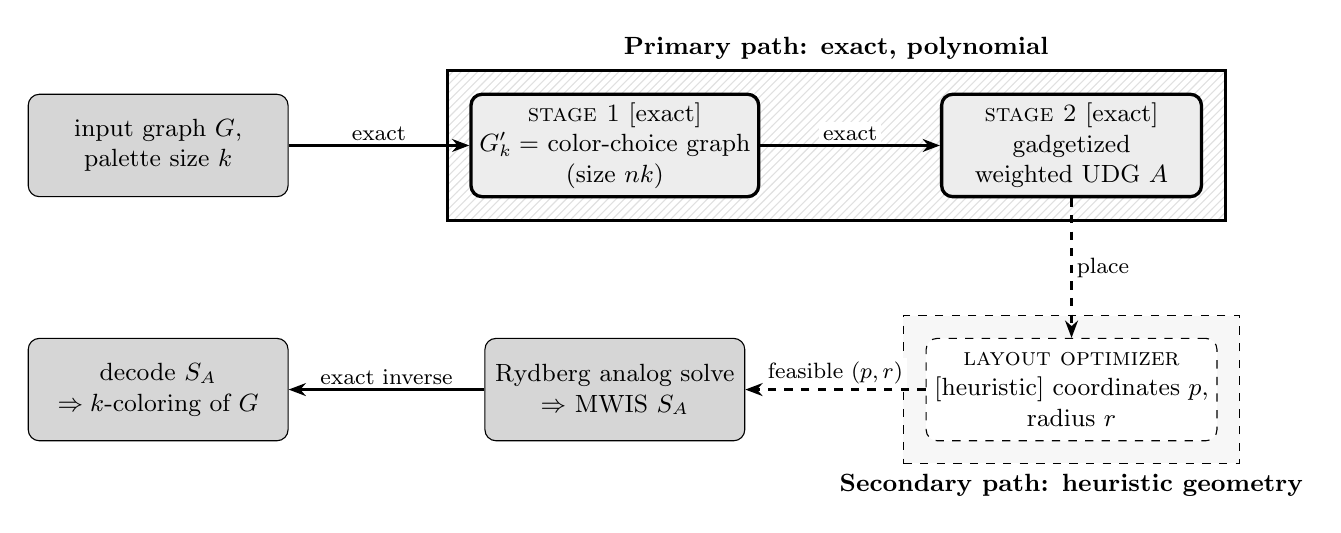
\begin{tikzpicture}[
  font=\small,
  box/.style={rectangle,draw,rounded corners,minimum width=33mm,minimum height=13mm,align=center,inner sep=3pt},
  exact/.style={box,very thick,fill=black!7},
  heur/.style={box,dashed,fill=white},
  io/.style={box,fill=black!16},
  ar/.style={-{Stealth[length=2.2mm]},thick},
  arh/.style={-{Stealth[length=2.2mm]},thick,dashed},
  lbl/.style={font=\footnotesize,fill=white,inner sep=1.5pt}
]
% ── top row (left to right) ────────────────────────────────────────────────
\node[io]    (G)  at (0,0)     {input graph $G$,\\ palette size $k$};
\node[exact] (Gp) at (5.8,0)   {\textsc{stage 1} [exact]\\ $G'_k=$ color-choice graph\\ (size $nk$)};
\node[exact] (A)  at (11.6,0)  {\textsc{stage 2} [exact]\\ gadgetized\\ weighted UDG $A$};
% ── bottom row (right to left) ─────────────────────────────────────────────
\node[heur]  (layout) at (11.6,-3.1) {\textsc{layout optimizer}\\ {[heuristic]} coordinates $p$,\\ radius $r$};
\node[io]    (solve)  at (5.8,-3.1)  {Rydberg analog solve\\ $\Rightarrow$ MWIS $S_A$};
\node[io]    (dec)    at (0,-3.1)    {decode $S_A$\\ $\Rightarrow k$-coloring of $G$};

\draw[ar] (G)  -- node[lbl,above]{exact} (Gp);
\draw[ar] (Gp) -- node[lbl,above]{exact} (A);
\draw[arh] (A)  -- node[lbl,right]{place} (layout);
\draw[arh] (layout) -- node[lbl,above]{feasible $(p,r)$} (solve);
\draw[ar] (solve)  -- node[lbl,above]{exact inverse} (dec);

\begin{scope}[on background layer]
  \node[draw,solid,very thick,pattern=north east lines,pattern color=black!12,
        fit=(Gp)(A),inner sep=8pt,
        label=above:{\textbf{Primary path: exact, polynomial}}] {};
  \node[draw,dashed,fill=black!3,fit=(layout),inner sep=8pt,
        label=below:{\textbf{Secondary path: heuristic geometry}}] {};
\end{scope}
\end{tikzpicture}}
\caption{The two-layer pipeline. Correctness depends only on the primary path (thick
borders, hatched panel); the secondary path (dashed borders) affects only hardware
feasibility and the quality of the analog solve.}
\label{fig:overview}
\end{figure}

% =============================================================================
\section{Primary path: exact gadgetized reduction}
\label{sec:gadget}
% =============================================================================

The primary path is the composition of two exact reductions:
\[
  \underbrace{G,k}_{\text{coloring}}
  \;\xrightarrow{\;\text{Stage 1}\;}\;
  \underbrace{G'_k}_{\text{MIS instance, size }nk}
  \;\xrightarrow{\;\text{Stage 2}\;}\;
  \underbrace{A=(\,p,r,w\,)}_{\text{weighted UDG}}
  \;\xrightarrow{\;\text{solve}\;}\;
  S_A
  \;\xrightarrow{\;\text{decode}\;}\;
  \text{coloring of }G.
\]

\subsection{\texorpdfstring{Stage 1: colorability $\to$ independent set}{Stage 1: colorability to independent set}}
\label{sec:col2is}

\begin{definition}[Color-choice graph]
\label{def:choice}
Given $G=(V,E)$ and palette size $k$, the \emph{color-choice graph} is the graph
$G'_k=(V',E')$ with unit weights, vertex set $V'=V\times\{1,\dots,k\}$, and edge set
$E'=E'_{\mathrm{choice}}\cup E'_{\mathrm{conflict}}$ where
\begin{align*}
  E'_{\mathrm{choice}}   &= \bigl\{\{(v,i),(v,j)\} : v\in V,\ 1\le i<j\le k\bigr\},
   &&\text{(a $k$-clique per vertex)}\\
  E'_{\mathrm{conflict}} &= \bigl\{\{(u,i),(v,i)\} : \{u,v\}\in E,\ 1\le i\le k\bigr\}.
   &&\text{(same-color conflicts)}
\end{align*}
Then $|V'|=nk$ and $|E'|=n\binom{k}{2}+mk$.
\end{definition}

\noindent $G'_k$ is the Cartesian product $G\,\square\,K_k$~\cite{HammackImrichKlavzar2011}:
the copies of $K_k$ are the choice cliques, and the copies of $G$ carry the conflict
edges.

Read $(v,i)\in V'$ as the \emph{slot} ``vertex $v$ takes color $i$''. The choice
cliques allow at most one slot per vertex, and the conflict edges forbid equal colors
at the two ends of an edge of $G$; nothing else is forbidden. An independent set of
$G'_k$ is therefore exactly a partial proper coloring of $G$
(Figure~\ref{fig:c4}\,(b)), total iff it has size $n$.

\begin{theorem}[Exactness of Stage 1]
\label{thm:col2is}
For every graph $G$ and every $k\ge 1$,
\[
  \indep(G'_k) = n \quad\Longleftrightarrow\quad G \text{ is } k\text{-colorable},
\]
and $\indep(G'_k)\le n$ always. The size-$n$ independent sets of $G'_k$ are in bijection with
the proper $k$-colorings of $G$.
\end{theorem}

\begin{proof}
For each $v$, the $k$ vertices $\{(v,i)\}_i$ form a clique
($E'_{\mathrm{choice}}$), so any independent set $S$ contains at most one slot per
original vertex; hence $|S|\le n$.

($\Leftarrow$) Let $c$ be a proper $k$-coloring. Put
$S=\{(v,c(v)):v\in V\}$, so $|S|=n$. $S$ is independent: it has exactly one slot
per vertex (no choice edge is internal), and for any $\{u,v\}\in E$ we have
$c(u)\ne c(v)$, so no conflict edge $\{(u,c(u)),(v,c(v))\}$ exists, because conflict
edges join only \emph{equal} color indices. Thus $\indep(G'_k)\ge n$, and combined
with $\indep(G'_k)\le n$ we get $\indep(G'_k)=n$.

($\Rightarrow$) Let $S$ be independent with $|S|=n$. By the choice-clique bound $S$
has exactly one slot per vertex, defining $c(v)=i$ where $(v,i)\in S$. For
$\{u,v\}\in E$, if $c(u)=c(v)=i$ then $\{(u,i),(v,i)\}\in E'_{\mathrm{conflict}}$
would be internal to $S$, contradicting independence. Hence $c$ is proper.

The two maps $c\mapsto S$ and $S\mapsto c$ are mutually inverse, giving the
bijection.
\end{proof}

The least $k$ with $\indep(G'_k)=n$ is $\chi(G)$; since $\chi(G)\le n$, binary search
finds it with $O(\log n)$ solves.

\paragraph{Restrictions.} Restrictions of the language (Section~\ref{sec:lang}) on
single vertices or pairs of vertices are independence constraints on $G'_k$, so
Theorem~\ref{thm:col2is} extends to them.

\begin{proposition}[Restrictions]
\label{prop:restrictions}
Let every vertex $v$ have a set $L(v)\subseteq\{1,\dots,k\}$ of allowed colors, and
let $D$ and $Q$ be sets of pairs of distinct vertices that must receive different and
equal colors, respectively. Delete from $G'_k$ every slot $(v,i)$ with $i\notin L(v)$;
add the edges $\{(u,i),(w,i)\}$ for every $\{u,w\}\in D$; and add the edges
$\{(u,i),(w,j)\}$ with $i\ne j$ for every $\{u,w\}\in Q$. The size-$n$ independent
sets of the resulting graph are in bijection with the proper $k$-colorings $c$ of $G$
such that $c(v)\in L(v)$ for every $v$, $c(u)\ne c(w)$ for every pair in $D$, and
$c(u)=c(w)$ for every pair in $Q$.
\end{proposition}

\begin{proof}
As in the proof of Theorem~\ref{thm:col2is}, a size-$n$ independent set holds one slot
per vertex and defines a proper coloring $c$. The deleted slots are exactly the
disallowed colors; an edge added for $\{u,w\}\in D$ joins two slots exactly when they
give $u$ and $w$ the same color; and an edge added for $\{u,w\}\in Q$ joins two slots
exactly when they give $u$ and $w$ different colors. Conversely, a coloring that
satisfies the restrictions selects no deleted slot and no two ends of an added edge.
\end{proof}

\noindent In the language, \texttt{precolor}, \texttt{allow} and \texttt{forbid}
define $L$, \texttt{differentColor} and \texttt{distinctOn} define $D$, and
\texttt{sameColor} defines $Q$. The restricted graph has at most $nk$ vertices, so
Stage~2 and the bounds of Section~\ref{sec:size} apply unchanged. The counting
restrictions \texttt{useAtMost}~$j$ and \texttt{useExactly}~$j$ are not of this form:
an independence constraint forbids pairs of slots, whereas \texttt{useAtMost} bounds
the number of distinct colors, and \texttt{useExactly} is not even preserved when
slots are removed from a selection. The checker therefore rejects
\texttt{useExactly}, and \texttt{useAtMost}~$j$ with $j<k$, on the exact path
(Section~\ref{sec:haskell}); \texttt{useAtMost}~$j$ with $j\ge k$ is vacuous.
Theorems~\ref{thm:gadget} and~\ref{thm:endtoend} below hold for the restricted graph,
with ``$k$-colorable'' read as ``$k$-colorable under the restrictions''. The robust
decoders of Section~\ref{sec:robust} guarantee only properness under restrictions,
since a fresh color may lie outside $L(v)$.

\subsection{\texorpdfstring{Stage 2: independent set $\to$ unit-disk MWIS}{Stage 2: independent set to unit-disk MWIS}}
\label{sec:gadgetize}

$G'_k$ is generally not a UDG. Stage~2 embeds it into a weighted UDG with the
copy/crossing construction of \citet{Nguyen2023}, which builds on the Rydberg MWIS
encoding of \citet{Pichler2018}. The construction is not a contribution of this
paper; we use it as a black box behind the following interface.

\begin{theorem}[Gadgetized embedding, after~\cite{Nguyen2023}]
\label{thm:gadget}
Let $F=(V_F,E_F)$ be an arbitrary (unweighted) graph. There is a
polynomial-time procedure $\mathsf{gadgetize}$ that maps $F$
to a weighted unit-disk graph $A=(p,r,w)$ on a grid, together
with a designated set of \emph{logical} atoms
$\ell:V_F\hookrightarrow V(A)$ and a constant $C\ge 0$, such that
\[
  \MWIS(A,w) = \indep(F) + C,
\]
and every maximum-weight independent set $S_A$ of $A$ restricts on the logical
atoms to a maximum independent set
$S=\ell^{-1}(S_A\cap \ell(V_F))$ of $F$. The number of atoms is at most
$4|V_F|^2$~\cite[Sec.~V\,A]{Nguyen2023}, so $|V(A)| = O\!\left(|V_F|^2\right)$ in the
worst case.
We instantiate the theorem only at $F=G'_k$, the color-choice graph of
Definition~\ref{def:choice}.
\end{theorem}

\citet{Nguyen2023} treat a vertex-weighted source; in our notation, their
construction gives $\MWIS(A,w)=\MWIS(F,w_F)+C$, and the pipeline uses only
$w_F\equiv1$. The target carries non-uniform weights: $2\gamma$ on copy-line atoms,
$4\gamma$ on the four interior atoms of each crossing gadget, and $\gamma+w_F(v)/2$
and $\gamma-w_F(v)/2$ on the first and last atom of each line, with $2w_F(v)\le\gamma$.

\paragraph{How the construction works.} Two atoms interact only when they are close,
so a long edge cannot be realized directly. Each vertex $v\in V_F$ becomes a
\emph{copy line}, a chain of atoms whose two lowest-energy configurations are the two
alternating patterns, so that the chain carries one bit $n_v$, readable at its first
atom, the logical atom $\ell(v)$. Each line is drawn as a vertical and a horizontal
segment, and the lines form an upper-triangular \emph{crossing lattice}. In the full
lattice, which Theorem~\ref{thm:gadget} describes, every pair of lines crosses exactly
once. A crossing receives a \emph{crossing gadget}, which lets the two lines pass
without coupling, if $\{u,v\}\notin E_F$, and a \emph{crossing-with-edge gadget},
which additionally forbids $n_u=n_v=1$, otherwise (Figure~\ref{fig:gadgets}). The
full lattice consists of $|V_F|(|V_F|-1)/2$ tiles of at most eight atoms each, and
\citet[Sec.~V\,A]{Nguyen2023} bound the total, including the copy-line atoms on the
boundary of the lattice, by $4|V_F|^2$. The lattice diagonal sets the blockade
radius, and the constant $C$ absorbs the fixed contribution of the ancillas. If the
lines are ordered so that each ends after meeting its last neighbor (a path
decomposition of $F$), pairs of lines that no longer meet need no crossing; this and
local simplification rules shrink the lattice on sparse
inputs~\cite[App.~A]{Nguyen2023}
(Sections~\ref{sec:size} and~\ref{sec:layouteval}). We take the gadgets and weights
verbatim from~\cite{Nguyen2023}.

\begin{figure}[tb]
\centering
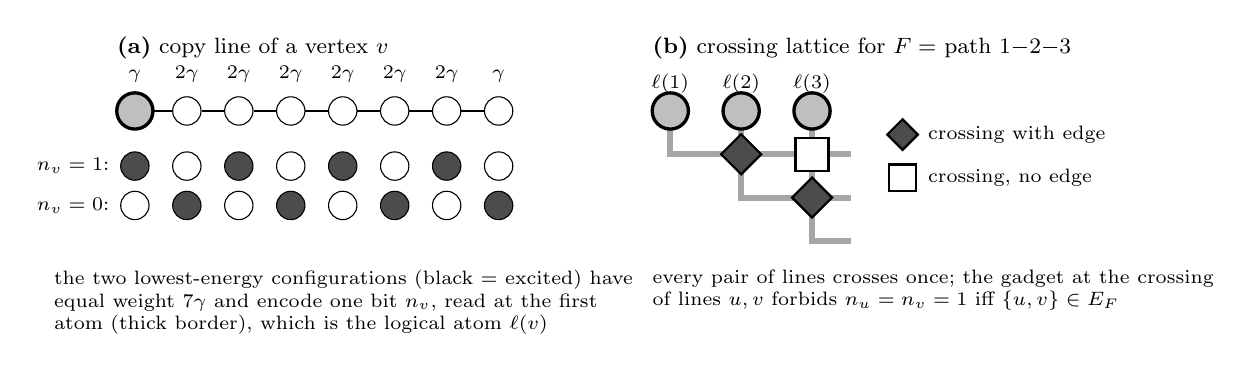
\begin{tikzpicture}[
  font=\small,
  atm/.style={circle,draw,minimum size=3.6mm,inner sep=0pt,fill=white},
  on/.style={circle,draw,minimum size=3.6mm,inner sep=0pt,fill=black!70},
  lg/.style={circle,draw,very thick,minimum size=4.6mm,inner sep=0pt,fill=black!25},
  cro/.style={rectangle,draw,thick,minimum size=4.2mm,inner sep=0pt,fill=white},
  cre/.style={diamond,draw,thick,minimum size=5.2mm,inner sep=0pt,fill=black!70},
  ln/.style={line width=2.2pt,black!35},
  wt/.style={font=\scriptsize,above=1.5pt}
]
% ── (a) one copy line ───────────────────────────────────────────────────────
\node[font=\footnotesize,anchor=west] at (-0.35,2.25)
  {\textbf{(a)} copy line of a vertex $v$};
\foreach \i/\w in {0/\gamma,1/2\gamma,2/2\gamma,3/2\gamma,4/2\gamma,5/2\gamma,6/2\gamma,7/\gamma}{
  \node[atm] (a\i) at (0.66*\i,1.45) {};
  \node[wt] at (a\i.north) {$\w$};
}
\draw (a0)--(a1)--(a2)--(a3)--(a4)--(a5)--(a6)--(a7);
\node[lg] at (a0) {};
\node[font=\scriptsize,anchor=east] at (-0.2,0.75) {$n_v=1$:};
\node[font=\scriptsize,anchor=east] at (-0.2,0.25) {$n_v=0$:};
\foreach \i in {0,...,7}{
  \pgfmathtruncatemacro\odd{mod(\i,2)}
  \ifnum\odd=0 \node[on] at (0.66*\i,0.75) {}; \node[atm] at (0.66*\i,0.25) {};
  \else        \node[atm] at (0.66*\i,0.75) {}; \node[on] at (0.66*\i,0.25) {}; \fi
}
\node[font=\scriptsize,align=left,anchor=north west] at (-1.15,-0.45)
  {the two lowest-energy configurations (black $=$ excited) have\\
   equal weight $7\gamma$ and encode one bit $n_v$, read at the first\\
   atom (thick border), which is the logical atom $\ell(v)$};

% ── (b) crossing lattice for F = path 1-2-3 ─────────────────────────────────
\begin{scope}[xshift=68mm]
\node[font=\footnotesize,anchor=west] at (-0.35,2.25)
  {\textbf{(b)} crossing lattice for $F=$ path $1{-}2{-}3$};
\draw[ln] (0,1.45)   -- (0,0.90)    -- (2.3,0.90);
\draw[ln] (0.9,1.45) -- (0.9,0.35)  -- (2.3,0.35);
\draw[ln] (1.8,1.45) -- (1.8,-0.20) -- (2.3,-0.20);
\foreach \i/\x in {1/0,2/0.9,3/1.8}{
  \node[lg] at (\x,1.45) {};
  \node[font=\scriptsize,above=3pt] at (\x,1.45) {$\ell(\i)$};
}
% crossings: horizontal segment of line i meets vertical segment of line j, i<j
\node[cre] at (0.9,0.90) {};   % lines 1,2: edge {1,2}
\node[cro] at (1.8,0.90) {};   % lines 1,3: no edge
\node[cre] at (1.8,0.35) {};   % lines 2,3: edge {2,3}
\node[cre,minimum size=4mm] at (2.95,1.15) {};
\node[font=\scriptsize,anchor=west] at (3.15,1.15) {crossing with edge};
\node[cro,minimum size=3.4mm] at (2.95,0.6) {};
\node[font=\scriptsize,anchor=west] at (3.15,0.6) {crossing, no edge};
\node[font=\scriptsize,align=left,anchor=north west] at (-0.35,-0.45)
  {every pair of lines crosses once; the gadget at the crossing\\
   of lines $u,v$ forbids $n_u=n_v=1$ iff $\{u,v\}\in E_F$};
\end{scope}
\end{tikzpicture}
\caption{The construction of Theorem~\ref{thm:gadget}, schematically. (a)~A copy
line of even length: interior atoms of weight $2\gamma$, end atoms of weight
$\gamma$, shifted to $\gamma\pm w_F(v)/2$ (first/last) in the weighted case so that
$n_v=1$ gains $w_F(v)$; the two alternating configurations carry one bit. (b)~The full crossing lattice: every pair of lines crosses
once, at a crossing-with-edge gadget (diamond) if the vertices are adjacent in $F$
and a plain crossing gadget (square) otherwise. Coordinates, gadget internals and
weights are those of~\citet{Nguyen2023}; Figure~\ref{fig:c4}\,(c) shows a complete
instance.}
\label{fig:gadgets}
\end{figure}

\paragraph{A combinatorial gadget.} Our implementation also builds a simpler,
non-geometric instance that satisfies the same interface except for the unit-disk
property. It is the weighted form of Poljak's reduction~\cite{Poljak1974}, which
subdivides every edge twice and raises the independence number by exactly the number
of edges.

\begin{lemma}[Edge-path gadget]
\label{lem:pathgadget}
Let $F=(V_F,E_F)$ be a graph, and let $A_4(F)$ be obtained from $F$ by replacing
every edge $\{u,v\}$ by a path $u - a_{uv} - b_{uv} - v$ through two new
vertices, with weight $1$ on $V_F$ and weight $2$ on every new vertex. Then
$\MWIS(A_4(F)) = \indep(F) + 2|E_F|$, and every maximum-weight independent set of
$A_4(F)$ restricts on $V_F$ to a maximum independent set of $F$. The instance has
$|V_F|+2|E_F|$ vertices.
\end{lemma}

\begin{proof}
Let $S_A$ be an independent set of $A_4(F)$, let $S=S_A\cap V_F$, and let $e(S)$
be the number of edges of $F$ with both ends in $S$. On each edge path at most one
of $a_{uv},b_{uv}$ is in $S_A$, and none is when $u,v\in S$; hence
$w(S_A)\le |S| + 2(|E_F|-e(S))$. Deleting one end of every edge inside $S$ leaves
an independent set $S'$ of $F$ with $|S'|\ge|S|-e(S)$, so
$w(S_A)\le |S'| + 2|E_F| - e(S)\le \indep(F)+2|E_F|-e(S)$. Conversely, for a
maximum independent set $I$ of $F$, choosing on every edge path the new vertex not
adjacent to an end in $I$ (at most one end is in $I$) gives an independent set of
weight $\indep(F)+2|E_F|$. So $\MWIS(A_4(F))=\indep(F)+2|E_F|$, and at an optimum
the bounds are tight: $e(S)=0$ and $|S|\ge\indep(F)$, so $S$ is a maximum
independent set of $F$.
\end{proof}

\noindent The type rule \rn{S2} of Section~\ref{sec:typing} records this offset
$C=2|E_F|$. In general, $A_4(F)$ is \emph{not} a unit-disk graph: a vertex of degree $d$
in $F$ is the center of an induced star $K_{1,d}$ in $A_4(F)$, which is impossible for
$d\ge6$ (Proposition~\ref{prop:starudg}). The metric
construction of Theorem~\ref{thm:gadget} is therefore what a device runs; $A_4(F)$ is
a checkable stand-in used by the implementation and the direct simulations of
Section~\ref{sec:gadgetval}.

\subsection{Decoding and end-to-end correctness}
\label{sec:decode}

Decoding composes the two inverses. Given a measured independent set $S_A$ of $A$,
restrict it to the logical atoms and apply $\ell^{-1}$ to obtain $S\subseteq V'$. The
readout is \emph{accepted} only if $S$ holds exactly one slot $(v,i)$ for every $v\in V$
and the map $c(v)=i$ is proper on every edge of $G$ (and, for a restricted instance,
satisfies the restrictions of Proposition~\ref{prop:restrictions}), an $O(nk+m)$ check; otherwise the shot is rejected, or repaired by the robust decoders of
Section~\ref{sec:robust}. A count of $n$ logical atoms is not enough, because the
gadget enforces the edges of $G'_k$ only at an optimum: for $K_2$ at $k=1$ the gadget
instance is the path $u-a-b-v$ with weights $1,2,2,1$, and its suboptimal independent
set $\{u,v\}$, of weight $2<3$, has $n=2$ logical atoms yet gives both ends of the edge
the same color. Optimal sets always pass (Theorem~\ref{thm:endtoend}\,(ii)).

\begin{theorem}[End-to-end exactness]
\label{thm:endtoend}
Let $A=\mathsf{gadgetize}(G'_k)$ for $G'_k$ the color-choice graph of $(G,k)$. Then:
\begin{enumerate}[label=(\roman*),leftmargin=2.2em]
  \item $\MWIS(A,w) = n + C$ if and only if $G$ is $k$-colorable.
  \item Any maximum-weight independent set of $A$ that contains $n$ logical atoms
        decodes, through $\ell^{-1}$ followed by the Stage-1 readout, to a proper
        $k$-coloring of $G$.
  \item The construction and the decoder both run in time polynomial in $n$ and
        $k$, and the decoder is an exact inverse of the construction; hence there
        is no chromatic-number inflation.
\end{enumerate}
\end{theorem}

\begin{proof}
By Theorem~\ref{thm:gadget} at $F=G'_k$, $\MWIS(A,w)=\indep(G'_k)+C$, and by
Theorem~\ref{thm:col2is}, $\indep(G'_k)\le n$ with equality iff $G$ is $k$-colorable;
this is (i). For (ii), a maximum-weight independent set of $A$ restricts to a maximum
independent set $S$ of $G'_k$, which the Stage-1 bijection reads off as a proper
coloring when $|S|=n$. For (iii), Stage~1 takes $O(nk^2+mk)$ time, matching
$|V'|=nk$ and $|E'|=n\binom{k}{2}+mk$; Stage~2 is polynomial by
Theorem~\ref{thm:gadget}; both readouts are linear; and exact inverses compose.
\end{proof}

\begin{remark}[Sources of uncertainty]
\label{rem:uncertainty}
Theorem~\ref{thm:endtoend} never assumes that the analog solve succeeds. The two
remaining risks are (a)~\emph{feasibility}, that is, whether $A$ fits within
$N_{\max}$ atoms and area $A_{\max}$ (Section~\ref{sec:size}), and (b)~\emph{solve
quality}, that is, whether the sweep returns a maximum-weight independent set or a
lighter one. Neither is a question about the correctness of the reduction. A returned
set can always be verified: a readout that passes the check above certifies a valid
coloring, whereas a failed check means only that no witness was found, not that none
exists. A non-colorability verdict therefore always needs an exact classical argument;
the decomposition of Section~\ref{sec:decomp} supplies one
(Theorem~\ref{thm:decsound}\,(ii)), and the device is used only to find colorings.
Section~\ref{sec:robust} shows that, on the combinatorial gadget, a suboptimal solve
costs at most one extra color per unit of lost weight.
\end{remark}

\subsection{Robustness to imperfect solves}
\label{sec:robust}

Every result so far assumes that the device returns an optimum. A sweep that is too
fast, or noise, leaves the array in a low-lying excited state instead, so the question
is how the decoder handles a near-optimal answer. For the combinatorial gadget of
Lemma~\ref{lem:pathgadget} the loss is additive: every unit of weight that the device
loses costs at most one extra color. A solution's
\emph{gap} is its distance to the optimum: $\MWIS(A)-w(S_A)$ for the gadget instance,
$\indep(G'_k)-|S|$ for $G'_k$, and the number of colors beyond $k$ for colorings of
$G$.

\begin{lemma}[Robust edge-path gadget]
\label{lem:robustgadget}
Let $S_A$ be an independent set of $A_4(F)$ with
$w(S_A)\ge\MWIS(A_4(F))-\varepsilon$. Deleting one end of every edge of $F$
whose two ends both lie in $S_A$ leaves an independent set $S'$ of $F$ with
$|S'|\ge\indep(F)-\varepsilon$, in time $O(|E_F|)$.
\end{lemma}

\begin{proof}
With $S=S_A\cap V_F$, the proof of Lemma~\ref{lem:pathgadget} gives
$w(S_A)\le|S'|+2|E_F|-e(S)\le|S'|+2|E_F|$, and
$\MWIS(A_4(F))=\indep(F)+2|E_F|$; hence $|S'|\ge w(S_A)-2|E_F|\ge
\indep(F)-\varepsilon$.
\end{proof}

\begin{proposition}[Robust Stage-1 decoding]
\label{prop:robuststage1}
Let $S$ be an independent set of $G'_k$ with $|S|=\indep(G'_k)-\varepsilon$, and
let $d=n-\indep(G'_k)$, so that $d=0$ exactly when $G$ is $k$-colorable
(Theorem~\ref{thm:col2is}). Coloring each vertex $v$ by the index of its selected
slot $(v,i)\in S$, and each vertex without a selected slot by a fresh color of its
own, produces in time $O(nk)$ a proper coloring of $G$ with at most $k+d+\varepsilon$
colors.
\end{proposition}

\begin{proof}
The choice cliques allow at most one selected slot per vertex, so the coloring is
well defined, and the conflict edges forbid two adjacent selected vertices from
sharing a color. A fresh color is used by one vertex only, so it never conflicts.
Exactly $n-|S|=d+\varepsilon$ vertices receive fresh colors.
\end{proof}

\begin{theorem}[End-to-end robustness]
\label{thm:robust}
Let the device return an independent set $S_A$ of $A_4(G'_k)$ with
$w(S_A)\ge\MWIS(A_4(G'_k))-\varepsilon$. Composing the decoders of
Lemma~\ref{lem:robustgadget} and Proposition~\ref{prop:robuststage1} produces in
polynomial time a proper coloring of $G$ with at most $k+d+\varepsilon$ colors,
so at most $k+\varepsilon$ if $G$ is $k$-colorable.
\end{theorem}

\begin{proof}
Lemma~\ref{lem:robustgadget} gives an independent set of $G'_k$ with gap at most
$\varepsilon$; Proposition~\ref{prop:robuststage1} decodes it.
\end{proof}

The guarantee is \emph{additive}, so a large offset does not weaken it.
\citet{Cazals2025} show that reductions to unit-disk MWIS do not preserve
approximation \emph{ratios}: because the optimum of the mapped instance is dominated
by the offset $C$, a relative gap on that instance may correspond to an arbitrarily
poor solution of the source. Theorem~\ref{thm:robust} gives the complementary
positive statement. Absolute gaps transfer one for one, so a solve that loses
$\varepsilon$ units of weight costs at most $\varepsilon$ extra colors, however large
$C$ is. Theorem~\ref{thm:robust} is an instance of the graded form of the type
system's decoder arrow (Refinement~D, Section~\ref{sec:refine}); both decoders and the
theorem itself, stated on the explicit edge list of $G'_k$, are mechanized in Rocq
(Section~\ref{sec:coq}). The metric case is open (Section~\ref{sec:future}).

\subsection{Size and feasibility bounds}
\label{sec:size}

\begin{proposition}[Atom budget]
\label{prop:atombudget}
For an instance $(G,k)$ with $|V|=n$, the gadgetized UDG $A$ uses
$nk\le|V(A)|\le4(nk)^2$ atoms, so $|V(A)|=O\bigl((nk)^2\bigr)$. The instance is
hardware-feasible only if $|V(A)|\le N_{\max}$ and the layout fits within $A_{\max}$
under spacing $d_{\min}$.
\end{proposition}

\begin{proof}
Stage 1 produces $|V'|=nk$ vertices, and Theorem~\ref{thm:gadget} at $F=G'_k$ gives at
most $4|V'|^2$ atoms. The lower bound is the logical-atom count.
\end{proof}

Measured against a device of a few hundred atoms~\cite{Wurtz2023}, the quadratic
blow-up is the practical bottleneck. It is not an artifact of this construction: under
the Exponential Time Hypothesis, any polynomial reduction from MWIS on arbitrary graphs
to MWIS on unit-disk graphs incurs a quadratic blow-up in vertex
count~\cite{Cazals2025}. Two techniques reduce the instance size.
\emph{Simplification}: repeatedly deleting vertices of degree $<k$, which can always be
colored last, leaves the $k$-core, and the $k$-core is $k$-colorable iff $G$ is.
Splitting at cut vertices into biconnected components is also safe, because the
colorings of the components can be permuted to agree on the cut vertices. For $k\le2$
no device is needed, since $2$-colorability is bipartiteness. \emph{Line ordering}: a
copy line need only extend until it has met every line it interacts with, and ordering
the lines of $F$ by a path decomposition shrinks the crossing lattice to
$O(|V_F|\,\mathrm{pw}(F))$~\cite[App.~A]{Nguyen2023}. We lift this bound to $G'_k$.

The \emph{vertex separation} of a vertex order $\pi$ is the largest number, over the
prefixes of $\pi$, of prefix vertices with a neighbor outside the prefix; its minimum
over all orders is the pathwidth~\cite{Kinnersley1992}. Write $\pi_k$ for the order of
$V'=V\times\{1,\dots,k\}$ that lists the $k$ slots of each vertex consecutively,
following $\pi$.

\begin{proposition}[Pathwidth bound]
\label{prop:pathwidth}
Let $\pi$ be a vertex order of $G$.
\begin{enumerate}[label=(\roman*),leftmargin=2.2em]
  \item If $\pi$ has vertex separation $s$, then $\pi_k$ has vertex separation at
        most $k(s+1)-1$; hence $\mathrm{pw}(G'_k)\le k(\mathrm{pw}(G)+1)-1$.
  \item \textup{(\citealp[App.~A]{Nguyen2023})} Let the lines of a graph $F$ be
        placed in a given order on a lattice of cells of constant size, such that
        (a)~each line is a vertical and a horizontal segment, and its horizontal
        segment ends in the column of its last neighbor in the order; (b)~a line
        occupies a row of cells only until that column, and freed rows are
        reused; and (c)~every crossing and every turn occupies one cell with a
        constant number of atoms, and simplification only removes atoms. If the
        order has vertex separation $s'$, the placement uses
        $O(|V_F|\,(s'+1))$ atoms.
\end{enumerate}
\noindent Consequently $G'_k$ placed by $\pi_k$ needs $O\bigl(nk^2(s+1)\bigr)$ atoms, linear in $n$
for bounded pathwidth and fixed $k$.
\end{proposition}

\begin{proof}
(i)~The neighbors of a slot $(u,c)$ are the other slots of $u$ and the slots
$(x,c)$ with $x$ adjacent to $u$. Consider a prefix of $\pi_k$ that ends inside
the slots of a vertex $v$: a prefix slot with a neighbor outside the prefix
belongs either to $v$ (at most $k-1$ slots) or to a vertex before $v$ with a
neighbor at or after $v$, and there are at most $s$ such vertices, so at most
$ks+k-1$ slots qualify. If the prefix ends after the last slot of $v$, only slots
of the at most $s$ vertices up to $v$ with a neighbor after $v$ qualify, at most
$ks$. The pathwidth statement follows because vertex separation and pathwidth
coincide~\cite{Kinnersley1992}.
(ii)~Call a line \emph{active} from its placement until its last neighbor has been
placed. At most $s'+1$ lines are active at once, so by (a) and~(b) the horizontal
segments use at most $s'+1$ rows of cells, and every vertical segment spans
$O(s'+1)$ cells. By~(a), the total horizontal length is the sum, over the cuts of
the order, of the lines active across the cut, which is at most $|V_F|\,s'$ cells.
Every crossing sits where a horizontal segment meets a vertical one, so there are at
most that many, and by~(c) each crossing and each turn contributes a constant number
of atoms.
\end{proof}

\noindent Conditions (a)--(c) describe the path-decomposition construction
of~\citet[App.~A]{Nguyen2023}; Section~\ref{sec:scaling} confirms the predicted
linear growth on its reference implementation~\cite{UnitDiskMapping}. The bound does
not contradict the lower bound of \citet{Cazals2025}, which concerns arbitrary graphs;
the pathwidth of an arbitrary graph can be linear in its order.

\subsection{\texorpdfstring{Worked example: $3$-coloring a small graph}{Worked example: 3-coloring a small graph}}
\label{sec:gadget-example}

\begin{example}
\label{ex:c4}
Let $G=C_4$ with vertices $v_1v_2v_3v_4$ and $k=3$ (Figure~\ref{fig:c4}). Stage~1
builds $G'_3$ with $|V'|=12$ slots and $|E'|=4\binom{3}{2}+4\cdot3=24$ edges: a choice
triangle per vertex and three conflict edges per edge of $C_4$. The proper coloring
$(1,2,1,2)$ corresponds to the independent set
$\{(v_1,1),(v_2,2),(v_3,1),(v_4,2)\}$ of size $n=4$, so $\indep(G'_3)=4$ and $C_4$ is
$3$-colorable; at $k=1$ the same construction gives $\indep(G'_1)=2<4$, correctly
reporting that $C_4$ is not $1$-colorable. Gadgetizing $G'_3$ gives a weighted UDG of
$285$ atoms, $12$ of them logical; an MWIS restricted to the logical atoms is an
independent set of size $4$ of $G'_3$, whose readout is a proper $3$-coloring such as
$(1,2,1,2)$. No inflation occurs at any step.
\end{example}

\begin{figure}[tb]
\centering
\resizebox{\linewidth}{!}{%
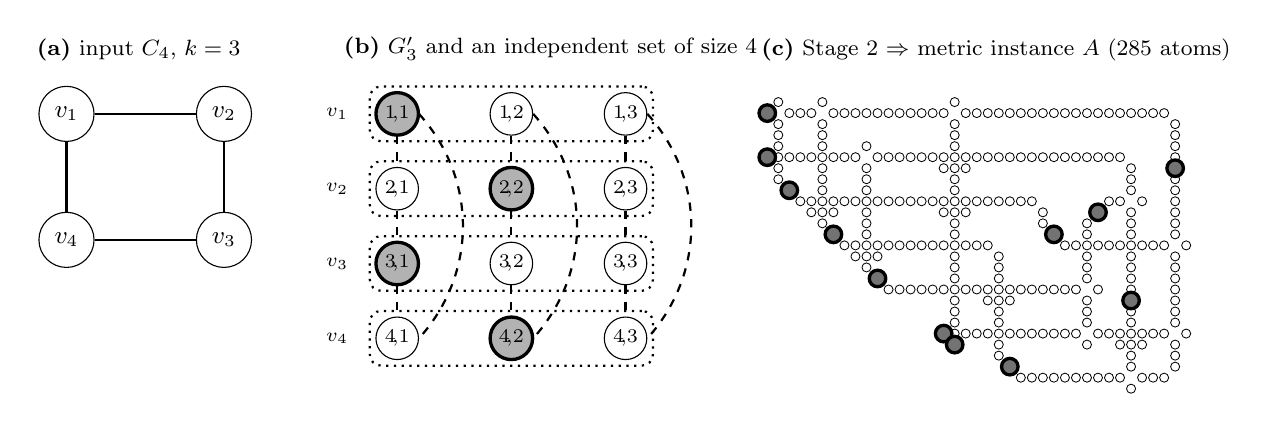
\begin{tikzpicture}[
  font=\small,
  v/.style={circle,draw,minimum size=7mm,inner sep=0pt,fill=white},
  slot/.style={circle,draw,minimum size=5.4mm,inner sep=0pt,fill=white,font=\scriptsize},
  sel/.style={circle,draw,very thick,minimum size=5.4mm,inner sep=0pt,fill=black!30,font=\scriptsize},
  ce/.style={thick},
  cf/.style={thick,dashed},
  cbox/.style={rounded corners,draw,dotted,thick,inner sep=2pt},
  ttl/.style={font=\footnotesize,anchor=south west}
]
% ─── (a) the input C4 ───────────────────────────────────────────────────────
\node[ttl] at (-0.5,2.75) {\textbf{(a)} input $C_4$, $k=3$};
\node[v] (p1) at (0,2.2)   {$v_1$};
\node[v] (p2) at (2.0,2.2) {$v_2$};
\node[v] (p3) at (2.0,0.6) {$v_3$};
\node[v] (p4) at (0,0.6)   {$v_4$};
\draw[ce] (p1)--(p2)--(p3)--(p4)--(p1);

% ─── (b) G'_3 with an independent set of size 4 ─────────────────────────────
\begin{scope}[xshift=42mm]
\node[ttl] at (-0.8,2.75) {\textbf{(b)} $G'_3$ and an independent set of size $4$};
\foreach \rr/\lab in {0/1,1/2,2/3,3/4}{
  \pgfmathsetmacro\yy{2.2-\rr*0.95}
  \foreach \cc in {1,2,3}{
    \pgfmathsetmacro\xx{(\cc-1)*1.45}
    \node[slot] (c\lab\cc) at (\xx,\yy) {$\lab\!,\!\cc$};
  }
  \node[font=\scriptsize,anchor=east] at (-0.5,\yy) {$v_\lab$};
  \node[cbox,fit=(c\lab1)(c\lab3)] {};
}
\foreach \cc in {1,2,3}{
  \draw[cf] (c1\cc)--(c2\cc); \draw[cf] (c2\cc)--(c3\cc); \draw[cf] (c3\cc)--(c4\cc);
  \draw[cf] (c1\cc.east) to[bend left=42] (c4\cc.east);
}
\node[sel] at (0,2.2)     {$1\!,\!1$};
\node[sel] at (1.45,1.25) {$2\!,\!2$};
\node[sel] at (0,0.3)    {$3\!,\!1$};
\node[sel] at (1.45,-0.65) {$4\!,\!2$};
\end{scope}

% ─── (c) the full metric gadget instance A (UnitDiskMapping.jl, our line order)
\begin{scope}[xshift=95mm]
\node[ttl] at (-0.8,2.75) {\textbf{(c)} Stage 2 $\Rightarrow$ metric instance $A$ ($285$ atoms)};
\def\u{0.14}
\begin{scope}[shift={(-0.6,2.35)},
  lt/.style={circle,draw,line width=0.3pt,minimum size=1.15mm,inner sep=0pt,fill=white},
  lg/.style={circle,draw,very thick,minimum size=2.1mm,inner sep=0pt,fill=black!55}]
\foreach \x/\y in {1/0,1/-2,1/-3,1/-4,1/-5,1/-6,1/-7,2/-1,2/-5,3/-1,3/-5,3/-9,4/-1,4/-5,4/-9,4/-10,5/0,5/-2,5/-3,5/-4,5/-5,5/-6,5/-7,5/-8,5/-9,5/-10,5/-11,6/-1,6/-5,6/-9,6/-10,7/-1,7/-5,7/-9,7/-13,8/-1,8/-5,8/-9,8/-13,8/-14,9/-1,9/-4,9/-6,9/-7,9/-8,9/-9,9/-10,9/-11,9/-12,9/-13,9/-14,9/-15,10/-1,10/-5,10/-9,10/-13,10/-14,11/-1,11/-5,11/-9,11/-13,11/-17,12/-1,12/-5,12/-9,12/-13,12/-17,13/-1,13/-5,13/-9,13/-13,13/-17,14/-1,14/-5,14/-9,14/-13,14/-17,15/-1,15/-5,15/-9,15/-13,15/-17,16/-1,16/-5,16/-6,16/-9,16/-10,16/-13,16/-17,17/0,17/-2,17/-3,17/-4,17/-5,17/-6,17/-7,17/-8,17/-9,17/-10,17/-11,17/-12,17/-13,17/-14,17/-15,17/-16,17/-17,17/-18,17/-19,17/-20,17/-21,18/-1,18/-5,18/-6,18/-9,18/-10,18/-13,18/-17,18/-21,19/-1,19/-5,19/-9,19/-13,19/-17,19/-21,20/-1,20/-5,20/-9,20/-13,20/-17,20/-18,20/-21,21/-1,21/-5,21/-9,21/-14,21/-15,21/-16,21/-17,21/-18,21/-19,21/-20,21/-21,21/-22,21/-23,22/-1,22/-5,22/-9,22/-17,22/-18,22/-21,23/-1,23/-5,23/-9,23/-17,23/-21,23/-25,24/-1,24/-5,24/-9,24/-17,24/-21,24/-25,25/-1,25/-5,25/-10,25/-11,25/-17,25/-21,25/-25,26/-1,26/-5,26/-17,26/-21,26/-25,27/-1,27/-5,27/-13,27/-17,27/-21,27/-25,28/-1,28/-5,28/-13,28/-17,28/-21,28/-25,29/-1,29/-5,29/-11,29/-12,29/-13,29/-14,29/-15,29/-16,29/-18,29/-19,29/-20,29/-22,29/-25,30/-1,30/-5,30/-13,30/-17,30/-21,30/-25,31/-1,31/-5,31/-9,31/-13,31/-21,31/-25,32/-1,32/-5,32/-9,32/-13,32/-21,32/-22,32/-25,33/-1,33/-6,33/-7,33/-8,33/-10,33/-11,33/-12,33/-13,33/-14,33/-15,33/-16,33/-17,33/-19,33/-20,33/-21,33/-22,33/-23,33/-24,33/-26,34/-1,34/-9,34/-13,34/-21,34/-22,34/-25,35/-1,35/-13,35/-21,35/-25,36/-1,36/-13,36/-21,36/-25,37/-2,37/-3,37/-4,37/-5,37/-7,37/-8,37/-9,37/-10,37/-11,37/-12,37/-14,37/-15,37/-16,37/-17,37/-18,37/-19,37/-20,37/-22,37/-23,37/-24,38/-13,38/-21}{\node[lt] at (\x*\u,\y*\u) {};}
\foreach \x/\y in {0/-1,0/-5,2/-8,6/-12,10/-16,16/-21,17/-22,22/-24,26/-12,30/-10,33/-18,37/-6}{\node[lg] at (\x*\u,\y*\u) {};}
\end{scope}
\end{scope}
\end{tikzpicture}}
\caption{Example~\ref{ex:c4} end to end. (a)~The input. (b)~$G'_3$ as a grid of
slots (row $=$ vertex, column $=$ color; dotted box $=$ choice clique, edges not drawn;
dashed $=$ conflict), with the independent set decoding to $(1,2,1,2)$ shaded.
(c)~The metric gadget instance produced by the reference
implementation~\cite{UnitDiskMapping} under the optimized line order of
Section~\ref{sec:layouteval}: $285$ atoms on a $27\times39$ lattice, in which atoms at
most one lattice diagonal apart interact; the $12$ logical atoms are dark. Its
maximum-weight independent sets restrict to those of $G'_3$ (checked exactly).}
\label{fig:c4}
\end{figure}


% =============================================================================
\section{Secondary path: heuristic geometry and the layout optimizer}
\label{sec:heuristics}
% =============================================================================

Given a prescribed weighted graph $B$ (in this paper, always a gadget instance), the
\emph{geometric realization problem} asks for a placement $p$ of $V(B)$ and a radius
$r$ such that $\UDG(p,r)$ equals the prescribed adjacency $E(B)$, subject to pairwise
spacing at least $d_{\min}$, $r\le r_{\max}$, and area at most $A_{\max}$. A
\emph{geometric heuristic} runs in polynomial time and may fail to find such a
placement; when it fails, it reports infeasibility instead of returning a placement
whose realized adjacency differs from $E(B)$. We first show that a geometric
supergraph cannot preserve the chromatic number in general, and then give the
heuristics and the role they play in Stage~2.

\subsection{Why geometric supergraphs cannot bound inflation}
\label{sec:impossibility}

\begin{definition}[Safe supergraph; false edges]
\label{def:safesuper}
A UDG $H=\UDG(p,r)$ on the vertex set $V$ of $G$ is a \emph{safe supergraph} of $G$ if
$E(G)\subseteq E(H)$; its \emph{false edges} are $\Efalse=E(H)\setminus E(G)$.
\end{definition}

\begin{proposition}[Safety $\Rightarrow$ decoder correctness]
\label{prop:safety}
If $E(G)\subseteq E(H)$ and $\kappa$ is a proper coloring of $H$, then $\kappa$
restricted to $V$ is a proper coloring of $G$. Consequently
$\chi(G)\le\chi(H)$.
\end{proposition}

\begin{proof}
Every edge of $G$ is an edge of $H$, so the endpoints receive distinct colors
under $\kappa$. The inequality follows since a proper coloring of $H$ is one of
$G$.
\end{proof}

Safe supergraphs therefore never lower $\chi$. The difficulty lies in the other
direction.

\begin{lemma}[Neighborhood packing in a UDG]
\label{lem:packing}
For every unit-disk graph $H=\UDG(p,r)$ and every vertex $v$ of $H$,
$\indep(H[N(v)])\le 5$.
\end{lemma}

\begin{proof}
Write $c=p(v)$, and suppose that $x_1,\dots,x_6$ in the closed disk $D$ of radius $r$
about $c$ are pairwise more than $r$ apart. No $x_i$ equals $c$, since $c$ is within
$r$ of every point of $D$. Sorting the $x_i$ by angle about $c$, some two consecutive
points $a,b$ subtend an angle $\theta=\angle\,acb\le 60^\circ$; assume
$\lVert c-a\rVert\le\lVert c-b\rVert$. In the (possibly degenerate) triangle $abc$
the angles at $a$ and $b$ sum to $180^\circ-\theta\ge120^\circ$, and the angle at $a$
is at least the angle at $b$, since it faces the longer side; hence it is at least
$60^\circ\ge\theta$. As the larger angle faces the larger side,
$\lVert a-b\rVert\le\lVert c-b\rVert\le r$, a contradiction.
\end{proof}

\begin{proposition}[Stars that are unit-disk graphs]
\label{prop:starudg}
In the plane, the star $K_{1,t}$ is a unit-disk graph if and only if $t\le 5$. Hence
the constant $5$ in Lemma~\ref{lem:packing} is sharp.
\end{proposition}

\begin{proof}
For $t\le5$, place the center at $c$ and $t$ leaves at
$c+r(\cos\frac{2\pi j}{5},\sin\frac{2\pi j}{5})$: every leaf is at distance $r$ from
$c$, and any two leaves are at distance at least $2r\sin(\pi/5)\approx1.176\,r>r$.
For $t\ge6$, the leaves would form an independent set of size $t>5$ inside $N(c)$,
contradicting Lemma~\ref{lem:packing}.
\end{proof}

\begin{theorem}[Supergraph inflation is unbounded]
\label{thm:impossibility}
There is a family of graphs with $\chi=2$ on which every safe UDG supergraph has
$\chi(H)\to\infty$. Concretely, for the star $K_{1,n}$,
\[
  \chi(K_{1,n}) = 2, \qquad \chi(H)\ \ge\ \Bigl\lceil \tfrac{n}{5}\Bigr\rceil+1
  \quad\text{for every safe UDG supergraph } H.
\]
\end{theorem}

\begin{proof}
$K_{1,n}$ is bipartite, so $\chi=2$. Let $H$ be a safe UDG supergraph with center
$c$ and leaves $L$, $|L|=n$. Safety forces every edge $\{c,\ell\}$ into $H$, so all
leaves lie within distance $r$ of $p(c)$, i.e.\ $L\subseteq N(c)$. In any proper
coloring of $H$, each color class is an independent set of $H$, hence an
independent set within $N(c)$, which by Lemma~\ref{lem:packing} has size $\le 5$.
Covering the $n$ leaves therefore needs at least $\lceil n/5\rceil$ color classes,
and $c$, adjacent to every leaf, one more. The bound is attained: put five groups of
at most $\lceil n/5\rceil$ leaves within $r/20$ of the points at distance $0.95r$
from $p(c)$ in the directions of Proposition~\ref{prop:starudg}; each group is a
clique, distinct groups are more than $r$ apart, and $\chi(H)=\lceil n/5\rceil+1$.
\end{proof}

\subsection{The layout loss and the heuristics}
\label{sec:seven}

For the gadget instance $A$ with prescribed adjacency $E_A$, the heuristics minimize
the \emph{realization} loss
\begin{equation}
\label{eq:layoutloss}
  L_{\mathrm{layout}}(p,r) =
  \underbrace{\sum_{\{u,v\}\in E_A}\!\!\max(0,d_{uv}-r)^2}_{\text{prescribed edges within }r}
  + \lambda\!\!\sum_{\{u,v\}\notin E_A}\!\!\max(0,r+\epsilon-d_{uv})^2
  + \mu\!\sum_{u\ne v}\max(0,d_{\min}-d_{uv})^2,
\end{equation}
where $d_{uv}=\|p(u)-p(v)\|_2$. The three terms penalize a prescribed edge longer
than $r$, a non-edge shorter than $r+\epsilon$, and a pair of atoms closer than
$d_{\min}$. The loss measures how far a placement is from realizing $E_A$ exactly; it
does not compare the placement with $G$. Seven heuristics initialize, run, repair
and tune this optimization. We give here the three that act on the lattice
construction evaluated in Section~\ref{sec:layouteval}; the other four apply to
free-form layouts and are in Appendix~\ref{app:freeform}.

\paragraph{H4 (Laplacian initialization).} Place vertex $v_i$ at
$p_0(v_i)=(\phi_2(i),\phi_3(i))$, using the Fiedler vector and the next Laplacian
eigenvector~\cite{Fiedler1973,Chung1997,Belkin2001}, which places adjacent atoms
close together~\cite{Fruchterman1991}; $O(|V(A)|^2)$ dense, $O(t\,|E_A|)$ for $t$
sparse iterations. On a lattice construction, the Fiedler vector alone orders the
copy lines.
\textbf{H5 (monotone local repair).} Push or pull offending pairs, accepting a move
only if it strictly decreases the potential
$\Phi=\sum_{\{u,v\}\in\mathcal X}\eta_{uv}$ over the violations $\mathcal X$, with
integer weights $\eta_{uv}\ge1$. As $\Phi$ is a nonnegative integer that every
accepted move decreases, at most $\Phi_0\le|V(A)|^2\max\eta$ moves occur.
\textbf{H7 (quality as evaluation).} Discrete measures such as realized non-edges and
decoded gap are piecewise constant in $(p,r)$ and give no useful gradient, so they are
used only to \emph{evaluate} and \emph{select} layouts.

\subsection{Why the heuristics are correctness-neutral}
\label{sec:role}

Used as a \emph{stand-alone supergraph backend}, the heuristics would place the
vertices of $G$ itself, color $H=\UDG(p,r)$, and restrict. By
Proposition~\ref{prop:safety} this never lowers $\chi$, but by
Theorem~\ref{thm:impossibility} nothing bounds how far it raises it; we retain this
backend only for comparison (Appendix~\ref{app:families} lists the families on which
it is exact). Inside Stage~2, by contrast, the gadget instance fixes the adjacency and
the weights exactly (Theorem~\ref{thm:gadget}); the heuristics only realize this
adjacency, minimizing atoms, crossings and chain length under the hardware
constraints. In this role the heuristics cannot affect correctness: a poor layout can
make the instance infeasible or make the ground state harder to reach, but it cannot
make a decoded answer wrong. For a lattice construction such as that of
Theorem~\ref{thm:gadget}, whose coordinates and radius are fixed once the copy lines
are ordered, the optimizer acts through that order (H4 initializes it, an H5-style
repair improves it, H7 selects by atom count; Section~\ref{sec:layouteval}), while
H1--H3 and H6 apply to free-form gadget layouts (Appendix~\ref{app:freeform}).

% =============================================================================
\section{Integrated pipeline and complexity}
\label{sec:pipeline}
% =============================================================================

The compiler chains the pieces of Figure~\ref{fig:overview}. It builds $G'_k$ in
$O(nk^2+mk)$ time (Theorem~\ref{thm:col2is}) and gadgetizes it in polynomial time
(Theorem~\ref{thm:gadget}), checking $N=|V(A)|\le\Nmax$, where $N=O((nk)^2)$
(Proposition~\ref{prop:atombudget}). It then lays out $A$: H4 initializes, H1--H2 run
for a budget of $T=\mathrm{poly}(N)$ steps followed by the feasibility check (raising
$r$ or rebuilding on failure), H3 and H5 repair, and H6 selects $(p,r^\star)$ with
$r^\star\le r_{\max}$ and area at most $A_{\max}$, at the costs given in
Section~\ref{sec:seven} and Appendix~\ref{app:freeform}. Finally, the device solves MWIS on $A$ at $(p,r^\star)$. The
decoder returns the Stage-1 readout of $S=\ell^{-1}(S_A)$ in $O(N)$ time if this
readout passes the check of Section~\ref{sec:decode}, and reports a solve failure
otherwise (Theorem~\ref{thm:endtoend}). The layout can affect feasibility, never
correctness. The compiler also never has to solve UDG \emph{recognition}, which is
NP-hard~\cite{Breu1998}, because it only realizes a prescribed adjacency.

\begin{corollary}[Polynomial compilation]
\label{prop:polytime}
With a fixed iteration budget $T=\mathrm{poly}(N)$, the compiler runs in time
polynomial in $n$ and $k$ for everything except the analog solve, and emits a hardware
instance of $O((nk)^2)$ atoms together with an exact decoder.
\end{corollary}

\begin{proof}
Each step is polynomial in $N=O((nk)^2)$ and $T$: $O(TN^2)$ for H1--H2,
$O(N\Delta^2)$ per H3 pass, at most $\Phi_0=O(N^2\max\eta)$ H5 moves, and
$O(N^2\log N)$ for H6. Exactness of the decoder is Theorem~\ref{thm:endtoend}.
\end{proof}

% =============================================================================
\section{Related work}
\label{sec:related}
% =============================================================================

\paragraph{Graph coloring and unit-disk graphs.} Deciding $k$-colorability is
NP-complete for $k\ge3$~\cite{Karp1972,GareyJohnson1979}, and $\chi$ is hard even to
approximate~\cite{Zuckerman2007}. It has been studied through the chromatic polynomial~\cite{Tutte1954}
and topological methods~\cite{Lovasz1978}; the Mycielskians~\cite{Mycielski1955} of our benchmark
(Section~\ref{sec:dimacs}) are the standard triangle-free graphs of large $\chi$.
Practical colorings come from greedy orderings~\cite{Welsh1967} and
DSATUR~\cite{Brelaz1979}; the clique number gives the lower bound
$\omega(G)\le\chi(G)$~\cite{West2001} and is itself NP-hard to compute~\cite{Bomze1999}.
UDGs are the intersection graphs of unit disks~\cite{Clark1990UDG}. Recognizing them is
NP-hard~\cite{Breu1998,KangMuller2012}, which is why we never try to realize the input
graph exactly. On UDGs themselves, coloring and maximum independent set admit simple
constant-factor approximation heuristics~\cite{Marathe1995}. Distance-based adjacency
also constrains colorings: some unit-distance graphs already have
$\chi=4$~\cite{MoserMoser1961}. Our two packing bounds
(Lemma~\ref{lem:packing}, Proposition~\ref{prop:hwclique}) are proved in full; the
planar packing density~\cite{FejesToth1953} would only sharpen a constant.

\paragraph{Rydberg MWIS and gadgetized reductions.} The identification of the
blockade ground state with UDG--MWIS is due to \citet{Pichler2018}, demonstrated on
hundreds of atoms by \citet{Ebadi2022} and with site-resolved weights by
\citet{deOliveira2025}. \citet{Nguyen2023} introduced the copy and crossing gadgets that
encode MWIS on an \emph{arbitrary} graph as MWIS on a weighted lattice UDG with at
most quadratic overhead, a known offset and a structural decoder; ancilla chains
acting as ``quantum wires'' serve a similar purpose~\cite{Kim2022}.
\citet{Cazals2025} prove the ETH-conditional quadratic lower bound for such reductions,
the counterpart of our size wall, and propose a linear-overhead divide-and-conquer
heuristic. Our primary path composes the classical colorability$\to$MIS reduction with
\citet{Nguyen2023}. We take the atom budget, field and spacing of QuEra's
Aquila~\cite{Wurtz2023} as reference device constraints, but we have not run the
gadget instances on it (Section~\ref{sec:discussion}). \citet{Angkhanawin2026} instead color a natively embedded UDG directly, using
several Rydberg levels per atom as colors (shown numerically for $k=3$); this needs
multi-level control and a unit-disk input, whereas we target the two-level encoding
and arbitrary graphs. The platform has been used both to study quantum phases on
256 atoms~\cite{Ebadi2021} and as a gate-model processor~\cite{Graham2022}. Photonic
devices have shown a sampling advantage~\cite{Madsen2022}; variational algorithms are
surveyed in~\cite{Cerezo2021} and the near-term setting in~\cite{Preskill2018}.

\paragraph{Layout and decomposition.} The layout optimizer uses standard tools in a
\emph{correctness-neutral} role: Laplacian eigenvectors~\cite{Chung1997,Fiedler1973}
and eigenmaps~\cite{Belkin2001}, force-directed drawing~\cite{Fruchterman1991},
multidimensional scaling~\cite{Kruskal1964}, simulated annealing~\cite{Kirkpatrick1983} and tabu search~\cite{Glover1997}. Chordal
graphs admit clique separators~\cite{Dirac1961}, which Tarjan's
decomposition~\cite{Tarjan1985} turns into a divide-and-conquer schedule; for clique
separators our \rn{Stitch} rule needs no boundary search. Tree-width and graph
minors~\cite{RobertsonSeymour1986} explain why coloring is tractable at bounded
width~\cite{ArnborgProskurowski1989}, and decompositions of fixed width can be found in
linear time~\cite{Bodlaender1996}. Our separator search is exhaustive: it tries
vertex sets of increasing size, up to four, and among the separating sets of the
smallest size keeps one that minimizes the largest remaining component. What is new here is that the device budget
$4(wk)^2\le\Nmax$ appears as a \emph{typed} premise (Section~\ref{sec:refine}).

\paragraph{Reductions with backward maps.} A pair of a forward map on instances and a
backward map on solutions is a morphism of Blass's category of
problems~\cite{Blass1995} and the data of a Weihrauch reduction in computable
analysis~\cite{BrattkaGherardi2011}; our certified reductions add that the backward
map is total on optima. L-reductions~\cite{PapadimitriouYannakakis1991} and the other
approximation-preserving reductions~\cite{Crescenzi1997} constrain how the backward
map transfers solution quality, which our graded decoders record as types
(Refinement~D). Reductions have been mechanized at scale for
undecidability~\cite{Forster2020} and for NP-completeness, including the Cook--Levin
theorem~\cite{GaeherKunze2021}; our development is much smaller and specific to
reductions whose decoders are certified on optima.

\paragraph{Types, effects and verified compilation.} Our calculus belongs to the line
of type-and-effect systems that includes the polymorphic effects of Lucassen and
Gifford~\cite{LucassenGifford1988}, their development into a general
discipline~\cite{TalpinJouvelot1992,NielsonNielson1999}, and applications to resource
usage~\cite{IgarashiKobayashi2002} and information flow~\cite{VolpanoIrvineSmith1996}.
Our decoder grades resemble graded effects and
types~\cite{Katsumata2014,Gaboardi2016,Orchard2019}. Most effect systems approximate
what a program does when it runs; ours instead record guarantees about
answer-preserving reductions. The safety effect accumulates bounds on chromatic
inflation, and the decoder grade tracks how solution gaps propagate through the
stages. Verified compilers such as CompCert~\cite{Leroy2009} and, for quantum
circuits, VOQC~\cite{Hietala2021} are proved correct once for all inputs. Translation
validation~\cite{Pnueli1998} and certifying algorithms~\cite{McConnell2011} instead
check each output, as UNSAT-proof checkers such as DRAT-trim~\cite{Wetzler2014} do;
some of these checkers are themselves formally verified~\cite{Tan2021}. We combine the
two approaches: the reduction is proved once, and each verdict is checked.

% =============================================================================
\section{The coloring language and its certified-reduction type system}
\label{sec:lang}
% =============================================================================

The pipeline is the denotation of programs in a small coloring-specification
language. A type system enforces its correctness, and the types of this system
describe \emph{problem reductions} rather than data shapes. The object being typed is
the classical decoder-carrying reduction of Section~\ref{sec:bg-levin}; the $\totopt$
judgment below does not define a new notion of reduction. Typing adds three
consequences that the classical notion does not give by itself. First, decoders
compose together with their total-on-optima certificates, so end-to-end soundness is
obtained as a derivation rather than as a separate proof. Second, transforms are
\emph{graded} by their effect on the chromatic number and on solution gaps, so a
transform that may inflate $\chi$ cannot be used unnoticed where a transform that
does not inflate it is required. Third, the legal order of stages follows from typing
(Corollary~\ref{cor:order}). Base types state that a program is well-formed, whereas
problem-types state that a reduction is faithful. We build only the problem-types and
leave base types to a standard typed core.

\subsection{The surface language}
\label{sec:surface}

A program declares a \texttt{graph}; a \texttt{palette} of colors; optional
\texttt{restrictions} (precolorings, allow/forbid lists, equality constraints, color
budgets); a \texttt{transform}, which is either a pipeline of stages composed with
\texttt{>>>} or a \texttt{toUDG} transform into a unit-disk graph; an
\texttt{instance} that ties these together; and a \texttt{compute} query
(Figures~\ref{fig:grammar} and~\ref{fig:program}). Restrictions on single vertices
and on pairs are compiled into the color-choice graph
(Proposition~\ref{prop:restrictions}); the counting restrictions \texttt{useAtMost}
and \texttt{useExactly} are rejected on the exact path. The two transform modes correspond
to the two notions of transformation in this paper: \texttt{toUDG(exact)} requires a
faithful unit-disk realization, while \texttt{toUDG(boundedChi}~$P$\texttt{)} is the
supergraph path. Because a UDG supergraph on the same vertices cannot preserve $\chi$
in general (Theorem~\ref{thm:impossibility}), \texttt{boundedChi} promises only that
$P$ is not lowered, together with a bound on how far it rises when such a bound is
certified. The safety effects of Section~\ref{sec:safetyeff} grade this promise, and
the type system rejects stronger annotations instead of merely discouraging them.

\begin{figure}[tb]
\small
\begin{lstlisting}[basicstyle=\ttfamily\scriptsize]
Decl          ::= "graph" Id "=" GraphExpr | "palette" Id "=" PaletteExpr
                | "restrictions" Id "=" "{" { Restriction ";" } "}"
                | "transform" Id "=" TransformExpr
                | "instance" Id "=" InstanceExpr | "compute" Id "=" QueryExpr
InstanceExpr  ::= "color" GraphRef [ "using" PaletteRef ]
                  [ "subjectTo" RestrRef ] [ "via" TransformRef ]
TransformExpr ::= Stage { ">>>" Stage }
Stage         ::= "colorChoice" Nat | "gadgetize" | "layout" [ Id ] | "emit"
                | "toUDG" "(" TransformMode { "," TransformOption } ")"
                | "superUDG" | "compose" "[" TransformRefList "]" | TransformRef
TransformMode ::= "exact" | "boundedChi" Property
Property      ::= "kColorable" "(" Nat ")" | "chromatic" | "bipartite"
Restriction   ::= "precolor" Vertex ":" Color | "allow" Vertex ":" ColorList
                | "forbid" Vertex ":" ColorList | "sameColor" "(" V "," V ")"
                | "differentColor" "(" V "," V ")" | "useAtMost" Nat
                | "useExactly" Nat | "distinctOn" VertexList
QueryExpr     ::= "chromaticNumber" "(" GraphRef ")"
\end{lstlisting}
\caption{Core grammar of the coloring-specification language, as accepted by the
prototype parser of Section~\ref{sec:haskell} (elided: literals,
transform options, the \texttt{encodeColoring} shorthand, optional
\texttt{Id :: Type} signatures, lexical classes).}
\label{fig:grammar}
\end{figure}

\begin{figure}[tb]
\small
\begin{lstlisting}[basicstyle=\ttfamily\scriptsize]
graph gInput = graph { vertices=[1,2,3,4,5],
                       edges=[(1,2),(2,3),(3,1),(1,4),(3,5)] }
palette pNamed = colors [red, blue, green]
restrictions rMain = { precolor 1 : red; differentColor(1,2); useAtMost 3 }
transform tExact   = colorChoice 3 >>> gadgetize >>> layout >>> emit
transform tBounded = toUDG(boundedChi chromatic, keep=[1,2,3], trackOrigin=true)
instance inst1 = color gInput using pNamed subjectTo rMain via tExact
instance inst2 = color gInput using pNamed subjectTo rMain via tBounded
compute  chiInput = chromaticNumber(gInput)
\end{lstlisting}
\caption{A well-typed program (\texttt{src/examples/paper\_figure.udgc}).
\texttt{inst1} colors \texttt{gInput} with a $3$-palette under \texttt{rMain} through
the exact pipeline \texttt{tExact}, typed $\tCol\rightsquigarrow\tDev$; \texttt{inst2}
uses the supergraph transform \texttt{tBounded}, typed $\tCol\rightsquigarrow\tCol$
with effect $\monoeff$. The prototype checker accepts it with no errors.}
\label{fig:program}
\end{figure}

\subsection{Problem-types and the certified-reduction judgment}
\label{sec:sorts}

A \emph{problem-type} (sort) names a class of instances together with the indices
needed to state preservation:
\begin{align*}
A,B \;::=\;
&\ \tCol\langle n,k\rangle                       && \text{$k$-coloring instance, $n=|V|$}\\
&\ \tCol\langle n,k \mid \beta{:}\,B\rangle       && \text{boundary-precolored ($\beta$ proper on $B\subseteq V$)}\\
&\ \tIS\langle N\rangle\{P\}                      && \text{independent-set instance, $N$ nodes, refinement $P$}\\
&\ \tWIS\langle N,\,C\rangle                       && \text{weighted IS, $N$ atoms, additive offset $C$}\\
&\ \tUDG\langle N,\,r,\,d\rangle                   && \text{\emph{exactly} realized unit-disk inst.\ (radius $r$, spacing $d$)}\\
&\ \tUDGa\langle N,\,r,\,d \mid f\rangle           && \text{\emph{approximately} realized, $f$ residual false edges}\\
&\ \tDev\langle N\rangle \quad (N\le \Nmax)        && \text{device-feasible instance}
\end{align*}
Each sort $A$ carries a solution domain $\Sol(A)$ and a set $\mathrm{opt}(A)$ of
optimal solutions. The solutions of $\tCol$ are the $k$-colorings together with the
answer ``not $k$-colorable''; a coloring is optimal when it is proper, and the answer
is optimal when no proper $k$-coloring exists. The optima of $\tIS$ and $\tWIS$ are
their maximum (weight) independent sets in the standard sense.
Stage-1 exactness is recorded in the refinement on $\tIS$; the canonical refinement is
$P_{\mathrm{s1}} \equiv \bigl(\indep = n \iff G \text{ is } k\text{-colorable}\bigr)\wedge \indep\le n$.
The two unit-disk sorts separate exact from approximate layouts. $\tUDG$ is a placement
whose realized graph equals the prescribed gadget adjacency exactly. A layout with
false edges realizes a \emph{different} graph and receives the sort $\tUDGa$, which is
not a legal source for the exact decoder; the types therefore forbid reading an
answer off such a layout.
\begin{definition}[Decoder, total on optima]
A \emph{decoder} from $B$ to $A$ is a partial map
$\delta:\Sol(B)\rightharpoonup\Sol(A)$. It is \emph{total on optima},
$\totopt(\delta)$, if it maps every optimal solution of $B$ to an optimal solution
of $A$.
\end{definition}

\begin{definition}[Certified reduction]
The judgment $\vdash \tau : A \redto{\delta} B$ asserts that $\tau$ takes an
instance of $A$ to an instance of $B$, that $\delta$ is a decoder
$B\!\rightharpoonup\!A$ with $\totopt(\delta)$, and that any optimum $s^\star$ of
$B$ gives the answer to $A$ as $\delta(s^\star)$. Operationally: \emph{solve $B$
on the device, apply $\delta$, obtain the answer to $A$.}
\end{definition}

The rest of the calculus is built on this arrow: each stage rule introduces one
arrow, composition chains arrows, and the refinements add indices (grade, effect,
budget, slack).

\subsection{Per-stage typing rules and soundness}
\label{sec:typing}

The premises of the rules are \emph{proof obligations}, discharged once and for all
by the theorems of Section~\ref{sec:gadget}. Stage~1 is the color-choice reduction and
Stage~2 the gadget embedding with its static offset $C$; Stage~3 branches on whether
the layout realizes the adjacency exactly, and \rn{Fit} moves the instance onto the
hardware.
\[
  \irule{n=|V(G)| \quad k\ge 1}
        {\vdash \mathsf{colorChoice}_k : \tCol\langle n,k\rangle
          \redto{\mathsf{decodeColoring}} \tIS\langle nk\rangle\{P_{\mathrm{s1}}\}}
  \quad\rn{S1}
\]
\[
  \irule{C = 2\,|E(G'_k)| \quad N_A=|V(A)|}
        {\vdash \mathsf{gadgetize} : \tIS\langle N\rangle\{P\}
          \redto{\mathsf{decodeLogical}} \tWIS\langle N_A,\ C\rangle}
  \quad\rn{S2}
\]
\[
  \irule{\realizes(p,r) \quad \mathsf{spacing}(p)\ge d}
        {\vdash \mathsf{layout}(p,r): \tWIS\langle N,C\rangle
          \redto{\mathrm{id}} \tUDG\langle N,r,d\rangle}
  \quad\rn{S3-exact}
\]
\[
  \irule{\miss(p,r)=\varnothing \quad f=|\false(p,r)|>0}
        {\vdash \mathsf{layout}(p,r): \tWIS\langle N,C\rangle
          \rightsquigarrow \tUDGa\langle N,r,d \mid f\rangle}
  \quad\rn{S3-approx}
\]
\[
  \irule{N\le \Nmax}
        {\vdash \mathsf{emit} : \tUDG\langle N,r,d\rangle \redto{\mathrm{id}} \tDev\langle N\rangle}
  \quad\rn{Fit}
\qquad
  \irule{\vdash \tau_1 : A \redto{\delta_1} B \quad \vdash \tau_2 : B \redto{\delta_2} C}
        {\vdash \tau_2\circ\tau_1 : A \redto{\delta_1\circ\delta_2} C}
  \quad\rn{Comp}
\]
Rule \rn{S2} records the offset $C$ and the atom count $N_A$ of the gadget instance
$A$, which \rn{Fit} compares with $\Nmax$. The premises shown are those of the
combinatorial gadget of Lemma~\ref{lem:pathgadget}, which the implementation
elaborates, with $N_A=N+C$; for the metric construction of Theorem~\ref{thm:gadget},
$C$ and $N_A$ are that construction's own, and nothing else changes. \rn{S3-exact} carries the identity decoder
(geometry never relabels a solution); \rn{S3-approx} carries \emph{no} certified
decoder. The only exit from $\tUDGa$ is a metric \rn{Repair} step
($\tUDGa \redto{\mathsf{decodeRoute}} \tWIS$) that re-routes false edges through
copy/crossing gadgets, after which \rn{S3-exact} may be retried.
\begin{theorem}[Pipeline soundness]
\label{thm:typesound}
If $\vdash \Pi : \tCol\langle n,k\rangle \redto{\delta} \tDev\langle N\rangle$ is
derivable (so that $N\le\Nmax$ and every layer is realized exactly), then:
\begin{enumerate}[label=(\roman*),leftmargin=2.2em]
  \item for every device measurement $m$, if $\delta(m)$ is a coloring, it is a proper
        $k$-coloring of $G$;
  \item for every optimal measurement $m$, $\delta(m)$ is a proper $k$-coloring of $G$
        if $G$ is $k$-colorable, and the answer ``not $k$-colorable'' otherwise.
\end{enumerate}
\end{theorem}
\begin{proofsketch}
(i)~The Stage-1 decoder $\delta_{\mathrm{s1}}$ ends with the readout check of
Section~\ref{sec:decode}, which returns a coloring only if it is proper. (ii)~By
induction on the derivation, using \rn{Comp}: each arrow is answer-preserving with a
$\totopt$ decoder, and $\totopt$ decoders compose, so
$\delta=\delta_{\mathrm{s1}}\!\circ\delta_{\mathrm{s2}}\!\circ\mathrm{id}\circ\mathrm{id}$
maps an optimum bitstring back through $\tWIS$ (strip $C$) to a maximum independent
set of $G'_k$; the refinement $P_{\mathrm{s1}}$ says that it has size $n$ if and only
if $G$ is $k$-colorable. The only
non-identity geometric step, \rn{S3-exact}, has premise $\realizes(p,r)$
guaranteeing that the realized graph is $A$, so their optima coincide. The argument is
the meta-theorem of Theorem~\ref{thm:endtoend}, here read off the derivation.
\end{proofsketch}

\noindent Only part~(ii) assumes optimality, and optimality cannot be checked on a
device. The implementation therefore relies on part~(i) alone: an accepted readout is a
certified coloring, and a rejected readout is never reported as non-colorability
(Remark~\ref{rem:uncertainty}).

\begin{corollary}[Ill-ordered pipelines do not type]
\label{cor:order}
The three stage-ordering errors are rejected by the types alone, without a
separate analysis: \rn{S2} (\emph{gadgetize before colorChoice}) expects $\tIS$ but is
given $\tCol$; \rn{Fit} (\emph{emit before layout}) expects $\tUDG$ but is given
$\tWIS$; and \emph{reading an answer off a false-edged layout} has no $\totopt$
decoder out of $\tUDGa$ (only \rn{Repair}, which goes back to $\tWIS$). The device
sort can be reached only through $\tUDG$. A measured bitstring therefore reaches a
coloring only through a chain of $\totopt$ decoders that ends with the readout check,
so every accepted coloring is proper (Theorem~\ref{thm:typesound}\,(i)).
\end{corollary}

\subsection{Four refinements}
\label{sec:refine}

\paragraph{Refinement A: certificate grade.} A grade $g\in\{\mathsf{w},\chi\}$ on
coloring conclusions, with $\mathsf{w}\sqsubseteq\chi$, distinguishes a cheap
witness-relative certificate ($\tCol^{\mathsf{w}}$: a carried coloring $\kappa$
proves $\chi(G)\le|\kappa|$, the default) from an exact one ($\tCol^{\chi}$:
$\chi(G)=k$ with a discharged lower bound). All stage rules preserve the grade; only
an explicit $\mathsf{prove}_\chi$ step lifts $\mathsf{w}\!\Rightarrow\!\chi$.
Theorem~\ref{thm:typesound} holds at grade $\mathsf{w}$, so sound compilation does
not require knowing $\chi(G)$.

\paragraph{Refinement B: the safety effect.}
\label{sec:safetyeff}
The supergraph path rewrites $G$ on the same vertices by adding edges (decoded by
restriction), so such a transform $G\mapsto H$ carries a \emph{safety effect}
$s\in\{\safe,\asafe{c},\monoeff\}$: $\safe$ means $\chi(H)=\chi(G)$;
$\asafe{c}$ means $\chi(G)\le\chi(H)\le\chi(G)+c$; and $\monoeff$ means
$\chi(G)\le\chi(H)$. Each is introduced only by a premise that establishes its meaning:
\[
  \irule{\Efalse=\varnothing}{s=\safe}
  \qquad
  \irule{K\ \text{a clique of}\ G,\ |K|=\ell \quad
         \kappa\ \text{a proper coloring of}\ H,\ |\kappa(V)|=u}
        {s=\asafe{u-\ell}}
  \qquad
  \irule{E(G)\subseteq E(H)}{s=\monoeff}
\]
The first premise makes preservation trivial; the second bounds the increase by two
checkable witnesses, since $\chi(H)\le u$ and $\chi(G)\ge\ell$; the third is
Proposition~\ref{prop:safety}. For a general supergraph transform it is not known in
advance whether it adds any edge, so such a transform is typed $\monoeff$, or
$\asafe{c}$ once a coloring of $H$ and a clique of $G$ are supplied. Effects form a commutative monoid,
$\safe\oplus s=s$, $\asafe{c}\oplus\asafe{c'}=\asafe{c{+}c'}$ and $\monoeff\oplus
s=\monoeff$ for $s\ne\safe$, and their meanings compose along $\oplus$, as bounds
on increases add.

Because $\oplus$ sums bounds while the intermediate graphs depend on the order in
which transforms are applied, two orderings of the same transforms are type-equal only
if their accumulated effects and side conditions match. The bound $\sigma(G)\le5$
serves as a \emph{screen}, not as a premise of any rule. If $\sigma(G)>5$,
Lemma~\ref{lem:packing} forces a false edge inside an independent set
$I\subseteq N(v)$ of size $\sigma(G)$; hence $\safe$ is impossible and
$\chi(H)\ge1+\lceil\sigma(G)/5\rceil$. This lower bound forces inflation when
$\chi(G)\le\lceil\sigma(G)/5\rceil$, as for stars, but not for every graph with
$\sigma(G)>5$. The prototype nevertheless rejects the supergraph path when
$\sigma(G)>5$. This rejection is a conservative policy, not a soundness requirement,
since $\monoeff$ is sound for every supergraph and $\asafe{c}$ is sound for every
discharged witness pair.

\paragraph{Refinement C: decomposition (split/stitch).} Decomposition makes the
discipline substructural: pieces are resources, and a shared separator is a value the
pieces must agree on. A separator $S$ with pieces $G_i=G[S\cup C_i]$ of width
$w=\max_i|G_i|$ splits the goal into independently compiled subgoals:
\[
  \irule{S\ \text{separates}\ G \quad w=\max_i|G_i| \quad 4(wk)^2\le \Nmax}
        {\vdash \mathsf{split}_S : \tCol\langle n,k\rangle \Longrightarrow
           \{\,\tCol\langle |G_i|,k\mid\beta_i{:}S\rangle\,\}_{i=1}^{p}}
  \quad\rn{Split}
\qquad
  \irule{\forall i,\ \kappa_i\ \text{proper};\ \ \kappa_i|_S=\kappa_j|_S}
        {\vdash \mathsf{stitch} : \{\kappa_i\}_i \redto{\cup} \kappa\ \text{on}\ G}
  \quad\rn{Stitch}
\]
The typed budget $4(wk)^2\le\Nmax$, which is Proposition~\ref{prop:atombudget} applied
to one piece, makes the peak device size depend on the piece width $w$ rather than on
$n$ (the analogue of register spilling, with atoms in place of registers). For a
clique separator, a color-relabeling coercion discharges the agreement premise without
search; in general, discharging it requires a search over the $k^{|S|}$ boundary
table. For a $256$-atom device the premise admits only $wk\le8$.
\begin{theorem}[Decomposed soundness]
\label{thm:decsound}
Let \rn{Split} split $G$ at $S$ into pieces $G_i=G[S\cup C_i]$.
\begin{enumerate}[label=(\roman*),leftmargin=2.2em]
  \item If each piece is compiled by a derivation of Theorem~\ref{thm:typesound}
        and \rn{Stitch} applies, then $\kappa=\bigcup_i\kappa_i$ is a proper
        $k$-coloring of $G$, and every device instance has at most
        $4(wk)^2\le\Nmax$ atoms.
  \item If, for every proper $k$-coloring $\beta$ of $G[S]$, some piece $G_i$ has
        no proper $k$-coloring extending $\beta|_S$, then $G$ is not
        $k$-colorable.
\end{enumerate}
\end{theorem}

\begin{proof}
(i)~Every edge of $G$ lies inside some $G_i$, because $S$ separates the components
$C_i$; the $\kappa_i$ are proper and agree on $S$, so their union is proper.
(ii)~A proper $k$-coloring $\kappa$ of $G$ would restrict to a proper coloring
$\beta=\kappa|_S$ of $G[S]$ and to proper extensions $\kappa|_{G_i}$ of $\beta$ on
every piece, contradicting the hypothesis.
\end{proof}

\noindent Part~(ii) quantifies over every piece and boundary coloring; a device solve
returning no coloring does not establish it (Remark~\ref{rem:uncertainty}), so
Section~\ref{sec:decomp} decides each such leaf by an exact classical check.

\paragraph{Refinement D: graded decoders.} The $\totopt$ arrow specifies what a
decoder does with an optimum; its graded form specifies what the decoder does with
any other solution.
Give every sort a gap, the distance of a solution from the optimum
(Section~\ref{sec:robust}), and call a decoder $\delta:\Sol(B)\to\Sol(A)$
\emph{robust with slack transfer} $g$, a monotone function on $\N$, if
$\mathrm{gap}_A(\delta(s))\le g(\mathrm{gap}_B(s))$ for every $s$. Robust decoders
compose with their slack transfers:
\[
  \irule{\vdash \tau_1 : A \redtos{\delta_1}{g_1} B \quad
         \vdash \tau_2 : B \redtos{\delta_2}{g_2} C}
        {\vdash \tau_2\circ\tau_1 : A \redtos{\delta_1\circ\delta_2}{g_1\circ g_2} C}
  \quad\rn{Comp-g}
\]
On the combinatorial path the stage grades are $g_{\mathrm{S2}}(\varepsilon)=
\varepsilon$ for the edge-path gadget (Lemma~\ref{lem:robustgadget}),
$g_{\mathrm{S1}}(\varepsilon)=d+\varepsilon$ with $d=n-\indep(G'_k)$ for the
fresh-color Stage-1 decoder (Proposition~\ref{prop:robuststage1}, the gap of a
coloring being its number of colors beyond $k$), and the identity for \rn{S3-exact}
and \rn{Fit}. Rule \rn{Comp-g} then derives Theorem~\ref{thm:robust}, with
$g=\varepsilon\mapsto d+\varepsilon$, for the whole pipeline; Rocq proves this
instance as one theorem (Section~\ref{sec:coq}). A $\totopt$ decoder is the special case
that maps gap $0$ to gap $0$, so the graded arrow refines the certified-reduction
judgment rather than replacing it. The grade $\varepsilon\mapsto\varepsilon$ is the
second condition of an L-reduction~\cite{PapadimitriouYannakakis1991} with $\beta=1$.
Typing adds that the grade travels with the decoder through every stage, so that a
stage which does not preserve absolute gaps is visible as a grade not of the form
$\varepsilon\mapsto c+\varepsilon$.


% =============================================================================
\section{Implementation, mechanized proofs, and empirical validation}
\label{sec:eval}
% =============================================================================

Every numeric result below is reproduced by the scripts in the artifact, and every
theorem cited as machine-checked is closed under the global context (no axioms, no
\texttt{Admitted}).

\subsection{Mechanized correctness in Rocq}
\label{sec:coq}

We formalize the calculus of Section~\ref{sec:lang} in the Rocq Prover~9.0.0 (formerly
Coq), in seven modules that use no external libraries. A \emph{problem type} bundles a
solution set with an optimality predicate; a \emph{certified reduction}
$\mathsf{CRed}\,A\,B$ carries an executable decoder $B\rightharpoonup A$ together with
a total-on-optima certificate. Reductions and their certificates compose, and a
single generic soundness lemma is reused at every stage. Table~\ref{tab:coq} maps each rule
and theorem of the paper to its Rocq counterpart.

\begin{table}[tb]
\centering
\small
\begin{tabular}{@{}>{\raggedright\arraybackslash}p{0.20\linewidth}>{\raggedright\arraybackslash}p{0.40\linewidth}>{\raggedright\arraybackslash}p{0.33\linewidth}@{}}
\toprule
Paper & Rocq (module\,.\,name) & Machine-checked statement \\
\midrule
sorts; decoder; $\totopt$; arrow
  & \texttt{Sorts.Pcol}, \texttt{Pis}, \texttt{Pwis}, \texttt{Pudg}, \texttt{Pdev};
    \texttt{Problem.decoder}, \texttt{tot\_opt}, \texttt{CRed}
  & definitions \\
\rn{Comp}
  & \texttt{Problem.cred\_comp}, \texttt{comp\_tot\_opt}, \texttt{cred\_sound}
  & certificates compose; a target optimum decodes to a source optimum \\
\rn{S1}; Thm.~\ref{thm:col2is}
  & \texttt{Stages.S1}, \texttt{decodeColoring\_tot\_opt}, \texttt{stage1\_opt}
  & a maximum independent selection has size $n$ $\iff$ $k$-colorable \\
\rn{S2}
  & \texttt{Stages.gadgetize}, \texttt{decodeLogical\_tot\_opt}, \texttt{gadget\_mwis}
  & an optimum has the largest weight, $=n+C$ $\iff$ colorable; $C$, $N$ indices \\
\rn{S3-exact}; \rn{Fit}
  & \texttt{Stages.layout\_exact}, \texttt{Stages.emit}
  & premises \texttt{Realizes} and \texttt{N <= Nmax} (atom count) \\
Thm.~\ref{thm:typesound}
  & \texttt{Pipeline.pipeline\_accept\_sound}, \texttt{pipeline\_sound},
    \texttt{pipeline\_decision}
  & (i) every accepted readout is proper; (ii) an optimal readout decides
    colorability \\
Cor.~\ref{cor:order}; \rn{S3-approx}
  & \texttt{Pipeline.dev\_only\_via\_udg}, \texttt{no\_gadget\_before\_choice},
    \texttt{no\_emit\_before\_layout}, \texttt{no\_exit\_from\_udga}
  & ill-ordered compositions do not type-check (\texttt{Fail}); no step
    derivation \\
Refinement~A
  & \texttt{Effect.Grade}, \texttt{gle\_refl/trans/antisym}
  & grade order \\
Refinement~B
  & \texttt{Effect.eplus\_id\_l/r}, \texttt{eplus\_assoc}, \texttt{eplus\_comm},
    \texttt{respects\_comp}, \texttt{asafe\_intro}, \texttt{mono\_intro}
  & commutative monoid; meanings compose along $\oplus$; witnesses give
    $\asafe{u-\ell}$ \\
Lemmas~\ref{lem:pathgadget}, \ref{lem:robustgadget}
  & \texttt{Robust.gadget\_mwis\_value}, \texttt{gadget\_optimum\_restricts},
    \texttt{gadget\_robust}
  & $\MWIS(A_4(F))=\indep(F)+2|E_F|$; optima restrict to maximum IS; gap
    $\varepsilon$ decodes to gap $\le\varepsilon$ \\
Prop.~\ref{prop:robuststage1}; \rn{Comp-g}
  & \texttt{Robust.stage1\_robust}, \texttt{robust\_comp}
  & fresh-color decoder proper with excess $n-|S|$; graded decoders compose \\
Thm.~\ref{thm:robust}
  & \texttt{Robust.robust\_end\_to\_end}
  & gap $\varepsilon$ on $A_4(G'_k)$ decodes to a proper coloring with at most
    $d+\varepsilon$ fresh colors \\
Refinement~C; Thm.~\ref{thm:decsound}\,(ii)
  & \texttt{Certificate.check\_coloring\_sound}, \texttt{check\_refutation\_sound}
  & accepted coloring is proper; accepted refutation $\Rightarrow$ no $k$-coloring \\
\bottomrule
\end{tabular}
\caption{Correspondence between the paper and the Rocq development (\texttt{proof/} in
the artifact; Rocq~9.0.0, axiom-free). The deliberate departures from a one-for-one
correspondence are listed in Section~\ref{sec:coq}.}
\label{tab:coq}
\end{table}

\paragraph{Scope of the mechanization.} The development departs from a one-for-one
correspondence in four deliberate ways.
(i)~\emph{Stage~2 is mechanized at its interface}: a solution is a logical selection
paired with an ancilla occupancy, the decoder is the projection, and the offset $C$ and
the atom count $N$ are indices of the sort, so \texttt{gadget\_mwis} does not state
$C=2|E'|$. That value, Lemma~\ref{lem:pathgadget}, is proved in the separate
\texttt{Robust} model of $A_4(F)$ for an arbitrary edge list, together with its robust
form. \texttt{Robust} also builds the explicit edge list of $G'_k$ and proves
Theorem~\ref{thm:robust} as the single theorem \texttt{robust\_end\_to\_end}; this
explicit model is not connected to the interface sort of the pipeline, so the exact
chain and the robust chain are two results side by side.
(ii)~\emph{Layout and emit only unwrap solutions}: \texttt{Pwis}, \texttt{Pudg} and
\texttt{Pdev} have the same optima but distinct solution types indexed by the atom
count (and by $C$), so composing the stage reductions in a wrong order, or with
mismatched atom counts, is a type error in Rocq, recorded by \texttt{Fail} commands in
\texttt{Pipeline}. The geometric and atom-count premises of \rn{S3-exact} and \rn{Fit}
only restrict which pipelines are derivable.
(iii)~\emph{The choice clique is encoded}: the selection type
\texttt{Sorts.Sel := nat -> option nat} enforces at most one slot per vertex by
construction. The optima of $\tIS$ are maximum independent selections in the standard
sense, and \texttt{stage1\_opt} proves that a maximum has size $n$ if and only if $G$
is $k$-colorable. Restrictions (Proposition~\ref{prop:restrictions}) are not
mechanized; the property suite checks them (Section~\ref{sec:haskell}).
(iv)~\emph{Refinement~C is checked through its output}: \rn{Split} and \rn{Stitch}
are not mechanized as typing rules. Instead, every decomposition run emits a
certificate, which the checkers proved sound in \texttt{Certificate} accept or reject
(Section~\ref{sec:certs}). This gives a translation-validation
guarantee~\cite{Pnueli1998} for each run, not a proof about the procedure. The metric UDG construction of~\cite{Nguyen2023} is
measured and checked exactly on small instances (Section~\ref{sec:layouteval}), not
mechanized.

\subsection{The typed front end}
\label{sec:haskell}

The Haskell package \texttt{udg-color} (GHC~9.12) implements the surface pipeline: a
parser and AST; a checker that tracks each transform's sorts and safety effect,
enforces stage ordering by sort adjacency, and applies the atom-budget check of
\rn{Fit} and the $\sigma(G)\le 5$ gate; an elaborator that lowers well-typed programs,
restrictions included (Proposition~\ref{prop:restrictions}), through Stage~1 and the
combinatorial gadget; and an emitter that writes the device instance consumed
by the simulator. The Haskell decoders are not extracted from Rocq; a property suite
checks them against the brute-force oracle. The checker accepts the program of
Figure~\ref{fig:program} and rejects the stand-alone $\sigma(G)>5$ supergraph. The
prototype covers less than the calculus: it types every \texttt{boundedChi} or
\texttt{superUDG} transform $\monoeff$, since the witnesses that discharge
$\asafe{c}$ exist only after elaboration; it does not carry decoder terms in
transform types; it does not implement the grade of Refinement~A; and it does not
check the problem-type indices, which serve only as annotations.

The type system specifies thirteen ill-typed cases: (1)~a palette where a graph is
expected; (2, 3, 7)~a vertex outside $V$ in a restriction, an edge, or a
\texttt{keep}/\texttt{drop} list; (4)~a color outside the palette;
(5)~\texttt{useExactly} exceeding the palette; (6)~a restriction set reused on the
wrong graph; (8)~overlapping \texttt{keep}/\texttt{drop}; (9)~an \texttt{exact}
transform that drops vertices (\rn{S3-exact}); (10)~a weak transform used as a stronger
guarantee ($\mathsf{w}\not\sqsupseteq\chi$); (11)~a color in a vertex position; and
(12)~a UDG literal whose points and edges disagree; and (13)~a counting restriction
(\texttt{useExactly}, or \texttt{useAtMost} below the palette size) on the exact path.
Stage-ordering errors are rejected structurally (Corollary~\ref{cor:order}). The
prototype raises codes 1--5, 8, 9 and~13 and the stage-ordering and $\sigma>5$
rejections; codes 6, 7 and 10--12 are specified but not yet checked. All $15{,}338$
checks pass: a language suite of $4$ acceptance and rejection checks, and a property
suite of $15{,}334$ oracle checks (Stage-1 sizes, decoder round-trips, gadget offsets,
and the restriction encoding of Proposition~\ref{prop:restrictions} on every graph
with at most four vertices).

\paragraph{Slots, vertices and atoms.} We keep three counts apart. \emph{Slots} are
the $nk$ vertices of $G'_k$; Sections~\ref{sec:simval} and~\ref{sec:decomp} count
slots, and the $16$-slot ceiling is the simulator's $2^{nk}$ wall. The
$nk+2|E'|$ \emph{vertices of $A_4(G'_k)$} are counted only where that instance is
simulated directly (Sections~\ref{sec:robusteval} and~\ref{sec:gadgetval}).
\emph{Atoms} are the sites of a metric gadget instance (Table~\ref{tab:layouteval},
Figure~\ref{fig:scaling}), and only atoms are compared with a device budget. The
\rn{Fit} check of the prototype therefore reports an error only when the $nk$ logical
atoms alone exceed $\Nmax$, and reports that an instance fits only when the bound
$4(nk)^2$ of Proposition~\ref{prop:atombudget} is within $\Nmax$; otherwise, fit is
not established and has to be decided from the metric layout.

\subsection{Validating the reduction by Rydberg simulation}
\label{sec:simval}
\label{sec:random}

Our ideal-blockade simulator evolves the time-dependent Rydberg Hamiltonian under a
QuEra-style adiabatic protocol (ramp the Rabi drive $\Omega$ up and down while
sweeping $\Delta$ from negative to positive); the blockade is imposed as a hard energy
penalty on the edges of $G'_k$. Keeping the most-populated basis states that are
independent sets mimics the post-selection of repeated hardware shots. We compare the recovered
$|\MIS|$ with a brute-force oracle over the $(k{+}1)^n$ partial colorings. These runs
validate the implementation of Stage~1 and of the decomposition on $G'_k$; the
combinatorial Stage-2 gadget is simulated directly in Section~\ref{sec:gadgetval},
and the metric construction is measured in Section~\ref{sec:layouteval}.

We run ten named graphs ($P_4$, $C_4$, $C_5$, $K_3$, $K_4$, $K_{2,3}$, $K_{1,4}$, the
bull, the wheel $W_5$ and Petersen), each at $k=\chi$ and $k=\chi-1$. Petersen
($nk=30$) exceeds the simulator's wall; all $18$ simulated instances match the oracle,
and every colorable run decodes to a coloring verified to be proper. Because a small,
hand-picked suite risks selection bias, we repeat the comparison on
Erd\H{o}s--R\'enyi graphs $G(n,p)$ under a protocol fixed before the runs
(\texttt{benchmarks/run\_random.py}). Each cell has $20$ instances drawn from a fixed
seed, and none is discarded. Each instance is run at every $k\in\{\chi,\chi-1\}$ with
$k\ge1$ and $nk\le16$; one instance for which neither value qualified was run once at
$k=\lfloor16/n\rfloor$, where it is necessarily non-colorable. The densities lie on
both sides of the colorability threshold, so that both verdicts occur in every row.
Across $160$ instances and $286$ runs, every run matches the oracle, and all $130$
colorable runs decode to colorings verified to be proper (Table~\ref{tab:random}).

\begin{table}[tb]
\centering
\small
\begin{tabular}{@{}ccccccc@{}}
\toprule
$n$ & $p$ & instances & $k$ used & runs colorable\,/\,not & oracle $=$ sim & decoded proper \\
\midrule
$4$ & $0.5$  & $20$ & $1$--$3$ & $20$\,/\,$20$ & $40/40$ & $20/20$ \\
$5$ & $0.3$  & $20$ & $1$--$3$ & $20$\,/\,$17$ & $37/37$ & $20/20$ \\
$5$ & $0.5$  & $20$ & $1$--$3$ & $18$\,/\,$20$ & $38/38$ & $18/18$ \\
$5$ & $0.7$  & $20$ & $1$--$3$ & $10$\,/\,$20$ & $30/30$ & $10/10$ \\
$6$ & $0.2$  & $20$ & $1$, $2$ & $17$\,/\,$19$ & $36/36$ & $17/17$ \\
$6$ & $0.35$ & $20$ & $1$, $2$ & $12$\,/\,$20$ & $32/32$ & $12/12$ \\
$7$ & $0.2$  & $20$ & $1$, $2$ & $16$\,/\,$20$ & $36/36$ & $16/16$ \\
$8$ & $0.15$ & $20$ & $1$, $2$ & $17$\,/\,$20$ & $37/37$ & $17/17$ \\
\midrule
\multicolumn{2}{@{}l}{\textbf{total}} & $160$ & & $130$\,/\,$156$ & $286/286$ & $130/130$ \\
\bottomrule
\end{tabular}
\caption{Random $G(n,p)$ instances against the brute-force oracle (seed $20260901$;
raw data in \texttt{benchmarks/results/random.csv}). ``Runs'' counts simulated
$(G,k)$ pairs at $k=\chi$ (colorable) and $k=\chi-1$ (not colorable).}
\label{tab:random}
\end{table}

Stage-1 correctness is already established for all graphs and all $k$ by
Theorem~\ref{thm:col2is}, so these $304$ runs are \emph{regression checks}. They would
detect an implementation defect, including one that a structured suite could miss,
but they add no evidence for the reduction itself, which is proved. On the named
graphs, the cost of the simulator grows with its $2^{nk}$ state vector: under one
second up to $10$ slots, about $3$\,s at $12$, and about $55$\,s at the $16$-slot wall.
This wall is a limit of classical simulation, not the device budget $N_{\max}$; the
decomposition of Section~\ref{sec:decomp} avoids it.

\subsection{Imperfect solves}
\label{sec:robusteval}

To exercise Theorem~\ref{thm:robust} we make the simulator fail on purpose: the sweep
is shortened from $4$ to $1.2$ time units ($40$ steps instead of $90$--$160$), so that
many shots end in low-lying excited states. We sample $1000$ shots from the final
state of each run, discard those that violate the blockade (as hardware post-selection
would), and decode \emph{every} remaining shot with the robust decoders, including
suboptimal ones the exact pipeline would reject. Table~\ref{tab:robust} covers the
named graphs at $k=\chi$ on $G'_k$, and the combinatorial gadget array $A_4(G'_k)$ on
a chosen set of instances within the simulation wall
(\texttt{benchmarks/results/robust.csv}).

\begin{table}[tb]
\centering
\small
\setlength{\tabcolsep}{4.5pt}
\begin{tabular}{@{}llcccccccc@{}}
\toprule
level & instance & $k$ & size & shots & gap $0$ & gap $1$ & gap $\ge2$ & within bound & $k$-col.\ (greedy) \\
\midrule
$G'_k$ & $P_4$          & 2 & 8  & 1000 & 583 & 360 & 57  & 1000 & 873 \\
       & $C_4$          & 2 & 8  & 999  & 576 & 287 & 136 & 999  & 953 \\
       & $C_5$          & 3 & 15 & 993  & 187 & 586 & 220 & 993  & 993 \\
       & $K_3$          & 3 & 9  & 996  & 424 & 313 & 259 & 996  & 996 \\
       & $K_4$          & 4 & 16 & 1000 & 847 & 115 & 38  & 1000 & 1000 \\
       & $K_{2,3}$      & 2 & 10 & 999  & 490 & 294 & 215 & 999  & 939 \\
       & $K_{1,4}$      & 2 & 10 & 999  & 319 & 490 & 190 & 999  & 916 \\
       & Bull           & 3 & 15 & 988  & 208 & 535 & 245 & 988  & 686 \\
       & $W_5$          & 3 & 15 & 1000 & 194 & 433 & 373 & 1000 & 668 \\
\midrule
$A_4$  & $K_2$          & 2 & 12 & 956  & 394 & 493 & 69  & 956  & n/a \\
       & $K_2$          & 1 & 4  & 996  & 904 & 89  & 3   & 996  & n/a \\
       & $P_3$          & 1 & 7  & 993  & 533 & 419 & 41  & 993  & n/a \\
       & $K_3$          & 1 & 9  & 967  & 906 & 47  & 14  & 967  & n/a \\
       & $P_4$          & 1 & 10 & 988  & 792 & 173 & 23  & 988  & n/a \\
       & $C_4$          & 1 & 12 & 961  & 438 & 461 & 62  & 961  & n/a \\
\bottomrule
\end{tabular}
\caption{Deliberately imperfect solves (sweep shortened to $1.2$ time units; $1000$
shots per instance, blockade-violating shots discarded). ``Size'' counts the slots of
$G'_k$ or the vertices of $A_4(G'_k)$. ``Gap'' is the distance of a
shot from the optimum ($\indep(G'_k)-|S|$ on $G'_k$; $\MWIS(A)-w(S_A)$ on $A_4$).
``Within bound'' counts shots whose decoded coloring is proper and uses at most
$k+d+\varepsilon$ colors (Theorem~\ref{thm:robust}); on $A_4$ it also requires the
bound of Lemma~\ref{lem:robustgadget}. ``$k$-col.\ (greedy)'' counts shots from which
a greedy completion (try the $k$ palette colors before a fresh one) recovers a proper
$k$-coloring; it is not applicable (n/a) on $A_4$. Instances at $k=1$ on $A_4$ are not
$1$-colorable ($d>0$).}
\label{tab:robust}
\end{table}

All $14\,835$ decoded shots satisfy the bound of Theorem~\ref{thm:robust}, and every
$A_4$ shot satisfies Lemma~\ref{lem:robustgadget}, as the theorems require; this
result is again a regression check. The new information is in the other columns. With
the short sweep, only $19$--$85\,\%$ of the color-choice shots are optimal, and the
exact pipeline would discard the rest. The robust decoder turns every color-choice
shot into a proper coloring with at most $k+\varepsilon$ colors, and a greedy
completion recovers a proper $k$-coloring from $67$--$100\,\%$ of these shots. A suboptimal shot is
therefore still usable: each unit of lost weight costs at most one extra color, and in
most shots it costs none.

\subsection{Metric gadget instances and the layout optimizer}
\label{sec:layouteval}

We compute the gadget instance $A$ of Theorem~\ref{thm:gadget} for $G'_k$ with
UnitDiskMapping.jl~\cite{UnitDiskMapping}, the reference implementation
of~\cite{Nguyen2023}, in its weighted mode with default simplification rules. Since
coordinates and radius are fixed by the lattice once the \emph{order} of the copy
lines is fixed, the optimizer acts on that order (Section~\ref{sec:role}). We compare
three orders:
\emph{naive}, the input slot order $(v,c)\mapsto(v-1)k+c$; \emph{optimized}, the H4
order (slots sorted by the Fiedler vector of $G'_k$) followed by an H5-style repair
that accepts an adjacent transposition only if the atom count strictly decreases, so
that it terminates (H7: the objective is the measured count, never a surrogate); and
\emph{path decomposition}, the library's own order (exact branching for $nk\le16$, and
greedy with $50$ restarts above that size~\cite[App.~A]{Nguyen2023}), which serves as
a strong reference rather than as a baseline. An instance \emph{fits} if $|V(A)|\le\Nmax=256$ and its bounding box
lies within the $75\times76\,\mu$m field of QuEra's Aquila at its $4\,\mu$m minimum
spacing~\cite{Wurtz2023}; both are necessary conditions. To check that the counted
instances are correct, we solved MWIS on $A$ exactly for every instance with
$nk\le15$ under the naive and optimized orders, and confirmed
$\MWIS(A)=\MWIS(G'_k,w)+C$ for one uniform and two random source-weight vectors $w$;
all $24$ checks pass (\texttt{benchmarks/verify\_layout.jl}).

\begin{table}[tb]
\centering
\small
\setlength{\tabcolsep}{4pt}
\begin{tabular}{@{}lrrrrrrrrrc@{}}
\toprule
& & & \multicolumn{3}{c}{naive order} & \multicolumn{3}{c}{optimized order} & path & \\
\cmidrule(lr){4-6}\cmidrule(lr){7-9}
Instance & $nk$ & $|A_4|$ & atoms & cross. & box & atoms & cross. & box & dec. & fits \\
\midrule
$K_2$, $k{=}2$        & 4  & 12  & 29   & 1   & $10{\times}11$ & \textbf{19}   & 1   & $7{\times}7$    & 29   & yes \\
$P_4$, $k{=}2$        & 8  & 28  & 74   & 2   & $11{\times}26$ & \textbf{65}   & 3   & $11{\times}23$  & 74   & atoms only \\
$C_4$, $k{=}3$        & 12 & 60  & 314  & 16  & $27{\times}43$ & \textbf{285}  & 15  & $27{\times}39$  & 314  & no \\
$C_5$, $k{=}3$        & 15 & 75  & 398  & 19  & $27{\times}55$ & \textbf{371}  & 20  & $26{\times}55$  & 398  & no \\
$K_4$, $k{=}4$        & 16 & 112 & 793  & 61  & $51{\times}59$ & 688           & 50  & $43{\times}59$  & \textbf{666}  & no \\
Petersen, $k{=}3$     & 30 & 180 & 2074 & 140 & $63{\times}115$ & \textbf{1867} & 131 & $63{\times}115$ & 1882 & no \\
\texttt{myciel3}, $k{=}4$ & 44 & 336 & 5506 & 444 & $115{\times}171$ & \textbf{4019} & 279 & $83{\times}171$ & 4051 & no \\
\bottomrule
\end{tabular}
\caption{Metric gadget instances (UnitDiskMapping.jl~0.5.1) under three line orders.
``$|A_4|$'' is the number $nk+2|E'|$ of vertices of $A_4(G'_k)$, for comparison;
``cross.'' counts crossing gadgets; ``box'' is the bounding box in lattice sites;
``path dec.'' is the count under the library's path-decomposition order; bold marks
the smallest count per row. ``Fits'' refers to the best order and requires
$|V(A)|\le256$ and a box within Aquila's field at $4\,\mu$m spacing; ``atoms only''
means the budget is met but the field is not. Raw data:
\texttt{benchmarks/results/layout.csv}.}
\label{tab:layouteval}
\end{table}

Compared with the naive order, the optimized order reduces the atom count on every
instance, by $7$--$34\,\%$. It also uses fewer atoms than the path-decomposition order
on every instance except $K_4$ at $k=4$ ($688$ against $666$ atoms). Fewer atoms do not
always mean fewer crossings ($P_4$, $C_5$). The main limitation, however, is size.
Only $K_2$ and $P_4$ at $k=2$ meet the $256$-atom budget, and only $K_2$ also fits the
field of view. Even $C_4$ at $k=3$ needs $285$ atoms; Petersen at $k=3$ needs about
$1.9$ thousand and \texttt{myciel3} at $k=4$ about $4.0$ thousand. These counts make
the quadratic overhead of Proposition~\ref{prop:atombudget} concrete: on present
hardware the exact path is limited to very small instances, and the layout optimizer
improves the constant factor but not the growth rate.

\paragraph{Direct simulation of the combinatorial gadget.}
\label{sec:gadgetval}
The runs of Section~\ref{sec:simval} place the blockade on the edges of $G'_k$ and
never materialize a Stage-2 instance. We therefore also simulate the combinatorial
instance $A_4(G'_k)$ of Lemma~\ref{lem:pathgadget} itself, with the blockade on its
edges, on
the instances that fit within the classical simulation wall. For the single edge $K_2$ at $k=2$ the
$12$-vertex instance gives $\MWIS(A)=\indep(G'_k)+C=2+8=10$, and its logical vertices
decode to the proper coloring $a\!\to\!1,\ b\!\to\!2$; at $k=1$ the $4$-vertex
instance gives
$\MWIS(A)=1+2=3$, whose logical support of size $1<2$ correctly reports that $K_2$ is
not $1$-colorable. These two runs confirm the offset identity on the instance itself,
for one colorable and one non-colorable case. Larger instances exceed the wall, and
for them the identity rests on Lemma~\ref{lem:pathgadget}.

\paragraph{A geometric emulator check.}
\label{sec:bloqade}
We also ran the \texttt{bloqade-analog} emulator, which models the geometric
$C_6/r^6$ interaction instead of an abstract blockade, on a five-atom unit-disk
``bowtie'' (two triangles sharing an apex); it also returns maximum independent sets.
This single unweighted check does not show that the ideal-blockade model matches the
hardware; weighted metric instances with per-atom detunings are left for future work
(Section~\ref{sec:future}).

\subsection{Scaling with pathwidth}
\label{sec:scaling}

Proposition~\ref{prop:pathwidth} predicts that, under the lifted line order, the atom
count of bounded-pathwidth families grows linearly in $n$. We test this with the
reference implementation on paths, cycles, $2\times m$ ladders and $3\times m$ grids
with up to $40$ vertices at $k=3$ (so the color-choice graphs have up to $120$
vertices), and contrast them with complete graphs $K_n$, whose pathwidth is $n-1$
(\texttt{benchmarks/run\_scaling.jl}).

\begin{figure}[tb]
\centering
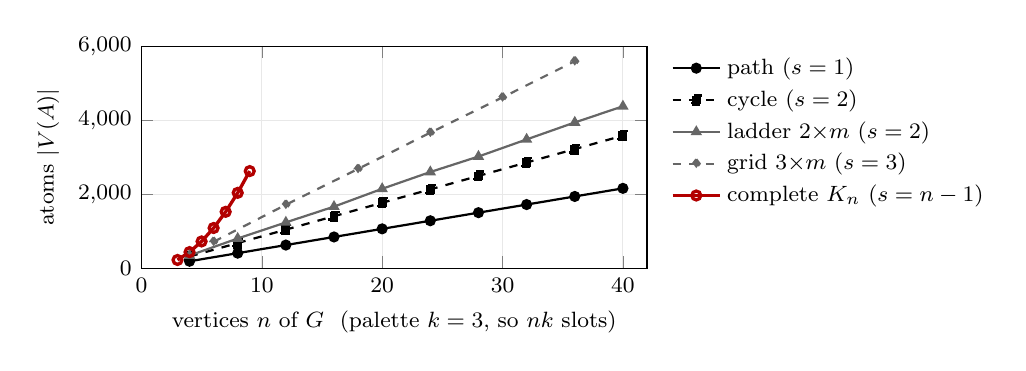
\begin{tikzpicture}
\begin{axis}[
  width=0.66\linewidth, height=4.4cm,
  xlabel={vertices $n$ of $G$ \ (palette $k=3$, so $nk$ slots)},
  ylabel={atoms $|V(A)|$},
  xmin=0, xmax=42, ymin=0, ymax=6000,
  grid=both, grid style={gray!18}, tick label style={font=\footnotesize},
  label style={font=\footnotesize},
  legend style={font=\footnotesize,at={(1.03,1)},anchor=north west,draw=none},
  legend cell align=left,
  mark size=1.6pt
]
\addplot[black,thick,mark=*] coordinates {(4,185)(8,404)(12,623)(16,842)(20,1061)(24,1280)(28,1499)(32,1718)(36,1937)(40,2156)};
\addplot[black,thick,dashed,mark=square*] coordinates {(4,314)(8,677)(12,1040)(16,1403)(20,1766)(24,2129)(28,2492)(32,2855)(36,3218)(40,3581)};
\addplot[black!60,thick,mark=triangle*] coordinates {(4,341)(8,800)(12,1236)(16,1662)(20,2144)(24,2598)(28,3017)(32,3479)(36,3938)(40,4374)};
\addplot[black!60,thick,dashed,mark=diamond*] coordinates {(6,712)(12,1713)(18,2681)(24,3662)(30,4616)(36,5593)};
\addplot[red!70!black,very thick,mark=o] coordinates {(3,220)(4,433)(5,721)(6,1084)(7,1522)(8,2035)(9,2623)};
\legend{path ($s=1$), cycle ($s=2$), ladder $2{\times}m$ ($s=2$), grid $3{\times}m$ ($s=3$), complete $K_n$ ($s=n-1$)}
\end{axis}
\end{tikzpicture}
\caption{Atoms of the metric gadget instance under the lifted line order
(UnitDiskMapping.jl). Bounded-pathwidth families grow linearly in $n$
(Proposition~\ref{prop:pathwidth}); complete graphs grow quadratically. The generic
bound $4(nk)^2$ is $57\,600$ at $n=40$.}
\label{fig:scaling}
\end{figure}

The measurements agree with the prediction (Figure~\ref{fig:scaling}). The atom
counts of paths and cycles grow by exactly $54.75$ and $90.75$ atoms per vertex (a
perfect linear fit); those of ladders and $3\times m$ grids grow by about $112$ and
$162$ atoms per vertex, with small residuals; and those of complete graphs grow
quadratically. In every case, the vertex separation of the lifted slot order is $ks$,
within the bound $k(s+1)-1$. At the largest sizes the instances are $8$ to $27$ times
smaller than $4(nk)^2$, and this ratio grows with $n$. On the bounded-pathwidth
families, the library's greedy path-decomposition order uses fewer atoms than the
lifted order only on the two smallest instances (by $4\,\%$ on the $2\times2$ ladder
and by $19\,\%$ on the $3\times2$ grid), and up to $24\,\%$ more elsewhere. On complete
graphs, for which every vertex order has the same separation, the library's order
uses $8$--$23\,\%$ fewer atoms throughout. Even with linear scaling, only the smallest
of these instances stay under a $256$-atom budget: a path at $k=3$ needs $185$ atoms at
$n=4$ and $404$ at $n=8$. Linear scaling does, however, remove the quadratic growth for
sparse structured inputs, and it suits the decomposition below, whose pieces are
small and structured.

\subsection{Avoiding the simulation wall by certified decomposition}
\label{sec:decomp}

A \emph{separator decomposition}, the classical counterpart of \rn{Split} and
\rn{Stitch}, avoids the $2^{nk}$ wall. Given a balanced vertex separator $S$, we
enumerate the proper colorings of $S$, solve each component plus its boundary as a
small piece, and stitch pieces that agree on $S$; when no separator is available, we
pin a free vertex and branch over its $k$ colors. The size of the largest piece
depends on the separator width, not on $n$. Each leaf is first given to the device; a
coloring that the device returns is a \emph{witness}, which is checked and then used.
If the device returns no coloring, which does not show that none exists
(Remark~\ref{rem:uncertainty}), an exact search over the leaf's at most $13$ slots
either finds a coloring (a \emph{device miss}) or proves that none exists. Pinning
never changes colorability, so the recursion is exact. A ``not $k$-colorable'' verdict
is therefore a classical proof, namely the boundary enumeration of
Theorem~\ref{thm:decsound}\,(ii) with exact leaf checks. The device supplies colorings,
never lower bounds.

Table~\ref{tab:decomp} reports four groups of runs. In the first group, choosing
$k>\chi$ raises the whole-instance $nk$ to as much as $192$, which would require a
monolithic state vector of $2^{192}$ amplitudes, while every simulated solve stays at
$\le13$ logical slots. This group exercises only the colorable direction, which a
palette larger than $\chi$ makes easy. The second group runs the same graphs at
$k=\chi$ and $k=\chi-1$, and the third adds further graphs, including the odd cycle
$C_{21}$ at $k=2$; the fourth group, the DIMACS Mycielski graphs, is discussed below.
Every verdict agrees with the known chromatic number. The device never missed a
colorable leaf: the exact check was needed only on leaves that have no coloring.

\paragraph{The DIMACS Mycielski benchmark.}
\label{sec:dimacs}
The Mycielskians \texttt{myciel3}--\texttt{myciel7} of the DIMACS coloring
suite~\cite{JohnsonTrick1996} are triangle-free graphs from a family whose chromatic
number grows without bound; on them the clique lower bound gives only $\chi\ge2$
($\omega=2$). Running \texttt{myciel3} in both directions certifies its chromatic
number exactly. The run at $k=\chi=4$ finds a proper coloring on the device. The run
at $k=3$ proves classically that no $3$-coloring exists: it exhausts the boundary
table, and every leaf on which the device finds no coloring is decided by the exact
check. This proof visits $158$ leaves in $106$\,s, including certificate generation;
the device colors $75$ of the leaves, and the other $83$ are certified infeasible. For
\texttt{myciel4} we run the feasible direction and find an optimal $5$-coloring; the
infeasible direction, which requires heavy backtracking, exceeds our time budget. In
these runs every simulated solve stays at $\le11$ logical slots, whereas monolithic
simulation would need state vectors of $2^{44}$ and $2^{115}$ amplitudes.
\texttt{myciel5} ($n=47$) and dense instances such as the queen graphs have large
separators, which prevent the decomposition from keeping the pieces small; these
instances are beyond our reach.

\begin{table}[tb]
\centering
\small
\setlength{\tabcolsep}{4.5pt}
\begin{tabular}{@{}lccccccccl@{}}
\toprule
Graph & $n$ & $m$ & $\chi$ & $k$ & whole $nk$ & max piece & calls & exact & verdict \\
\midrule
$C_{24}$ (cycle)      & 24 & 24 & 2 & 8  & 192 & 11 & 8  & 0  & proper ($5$ colors) \\
Ladder $2{\times}10$  & 20 & 28 & 2 & 8  & 160 & 11 & 10 & 0  & proper ($4$ colors) \\
Dodecahedral          & 20 & 30 & 3 & 8  & 160 & 13 & 7  & 0  & proper ($7$ colors) \\
Star $K_{1,12}$       & 13 & 12 & 2 & 10 & 130 & 11 & 12 & 0  & proper ($2$ colors) \\
Petersen              & 10 & 15 & 3 & 8  & 80  & 13 & 3  & 0  & proper ($6$ colors) \\
\midrule
$C_{24}$ (cycle)      & 24 & 24 & 2 & 2  & 48  & 12 & 4  & 0  & proper \\
                      &    &    &   & 1  & 24  & 7  & 1  & 1  & \textbf{not 1-colorable} \\
Ladder $2{\times}10$  & 20 & 28 & 2 & 2  & 40  & 12 & 6  & 0  & proper \\
                      &    &    &   & 1  & 20  & 11 & 1  & 1  & \textbf{not 1-colorable} \\
Dodecahedral          & 20 & 30 & 3 & 3  & 60  & 10 & 25 & 9  & proper \\
                      &    &    &   & 2  & 40  & 8  & 16 & 14 & \textbf{not 2-colorable} \\
Star $K_{1,12}$       & 13 & 12 & 2 & 2  & 26  & 3  & 12 & 0  & proper \\
                      &    &    &   & 1  & 13  & 2  & 1  & 1  & \textbf{not 1-colorable} \\
Petersen              & 10 & 15 & 3 & 3  & 30  & 10 & 4  & 1  & proper \\
                      &    &    &   & 2  & 20  & 8  & 10 & 8  & \textbf{not 2-colorable} \\
\midrule
Desargues             & 20 & 30 & 2 & 2  & 40  & 11 & 7  & 1  & proper \\
$C_{30}$ (cycle)      & 30 & 30 & 2 & 3  & 90  & 11 & 8  & 0  & proper \\
$C_{21}$ (odd)        & 21 & 21 & 3 & 2  & 42  & 12 & 17 & 9  & \textbf{not 2-colorable} \\
\midrule
\texttt{myciel3}      & 11 & 20 & 4 & 4  & 44  & 10 & 4   & 0  & proper \\
                      &    &    &   & 3  & 33  & 11 & 158 & 83 & \textbf{not 3-colorable} \\
\texttt{myciel4}      & 23 & 71 & 5 & 5  & 115 & 11 & 11  & 0  & proper \\
\bottomrule
\end{tabular}
\caption{Certified decomposition. First group: $k$ above $\chi$ to scale $nk$
(colorable direction only); second: the same graphs at $k=\chi$ and $k=\chi-1$;
third: further graphs; fourth: the DIMACS Mycielski graphs. ``Max piece'' is the
largest number of slots in a simulated piece, in which a precolored vertex has one slot
and a free vertex $k$ (so $K_{1,12}$ at $k=10$ gives $1+10=11$). ``Calls'' counts device
solves (each $\le13$ logical slots); ``exact'' counts the leaves on which the device
returned no coloring and which the exact check then decided. All of these leaves were
infeasible, so no colorable leaf was missed. Colorings are device witnesses checked classically;
every ``not colorable'' verdict is a classical certificate
(Theorem~\ref{thm:decsound}\,(ii)) accepted by the verified checker of
Section~\ref{sec:certs}. Raw data: \texttt{benchmarks/results/largenk.csv},
\texttt{decomp.csv} and \texttt{dimacs.csv}.}
\label{tab:decomp}
\end{table}

\subsection{Checkable certificates in both directions}
\label{sec:certs}

Theorem~\ref{thm:decsound} and the exact leaf checks make the decomposition's
verdicts correct; certificates make them \emph{checkable} by a small verified program,
independently of the solver, the simulator and the decomposition code. A colorable
verdict is certified by the coloring itself. A non-colorable verdict is certified by a
\emph{refutation}: a tree over color domains with four kinds of node.
$\mathsf{Split}\,v\,c$ branches on whether $v$ gets color $c$; $\mathsf{Restrict}\,W'$
narrows attention to a sub-piece $W'$; and the leaves $\mathsf{Clash}\,u\,v$ (an edge
whose ends are fixed to the same color) and $\mathsf{Empty}\,v$ (a vertex with no
color left) close a branch. A separator node of the decomposition becomes a chain of
$\mathsf{Split}$s over the separator; each boundary coloring then either clashes or is
followed by a $\mathsf{Restrict}$ to the piece that cannot be colored, which is the
structure of Theorem~\ref{thm:decsound}\,(ii). Each leaf piece is refuted by
$\mathsf{Split}$s down to clashes. The module \texttt{Certificate} defines the checker
as a Rocq function and proves \texttt{check\_refutation\_sound}: if
\texttt{check\_refutation}~$E$~$V$~$k$~$r$ returns \texttt{true}, then no map
$V\to\{0,\dots,k-1\}$ is a proper coloring of $(V,E)$; \texttt{check\_coloring\_sound}
states the analogous fact for colorings. Both
checkers are extracted to OCaml and wrapped in a parser of about $50$ lines; the
trusted base is the Rocq kernel, the extraction, the OCaml compiler and that parser.

All $26$ decomposition runs produce certificates: the $21$ rows of
Table~\ref{tab:decomp} and five further colorable runs recorded in
\texttt{decomp.csv} (Frucht at $k=3$, Heawood and Pappus at $k=2$, and second runs of
Petersen and the dodecahedral graph at $k=3$). The verified checker accepts all $26$,
each in under $20$\,ms. The two repeated runs write to the same file names as the
first runs, so the artifact keeps $24$ distinct certificate files. The $19$ colorable runs are certified by their
colorings; the $7$ non-colorable ones by refutations of $2$ to $794$ nodes: $2$--$3$
nodes for the $1$-colorability checks, $49$ for Petersen and $79$ for the dodecahedral
graph at $k=2$, $95$ for $C_{21}$ at $k=2$, and $794$ for \texttt{myciel3} at $k=3$,
whose certificate file is under $7$\,KB. Together with the $4$-coloring found on the
device, this refutation makes $\chi(\texttt{myciel3})=4$ a machine-checkable fact
whose lower bound does not depend on any quantum or simulated component. The design
is a certifying algorithm~\cite{McConnell2011}: the device searches for colorings,
classical certificates establish non-colorability, and in both directions trust rests
on a checker proved correct in Rocq rather than on the solver.

% =============================================================================
\section{Discussion and limitations}
\label{sec:discussion}
% =============================================================================

\paragraph{What is and is not guaranteed.} The reduction is exact, and its output can
be verified: a readout that passes the check of Section~\ref{sec:decode} is a
certified coloring, whatever the quality of the solve. Two things are not guaranteed:
that the device reaches the ground state, and that a large instance fits.
Theorem~\ref{thm:endtoend} separates both from correctness, and on the combinatorial
gadget a solve that misses the ground state still decodes within the bound of
Theorem~\ref{thm:robust}. A device failure is never read as a lower bound: every
non-colorability verdict in this paper either matches the oracle or is certified by a
refutation that the verified checker accepts. Section~\ref{sec:coq} states the scope
of the mechanization.

\paragraph{The size wall.} For devices of a few hundred atoms~\cite{Wurtz2023}, the
$O((nk)^2)$ atom count is the binding constraint; under the Exponential Time
Hypothesis, a quadratic overhead is unavoidable for reductions of this
kind~\cite{Cazals2025}. With the reference construction, only very small instances
meet a $256$-atom budget ($nk\le8$ in Table~\ref{tab:layouteval}, and $nk=12$ for a
path), and the classical simulator stops near $16$ slots. Three techniques reduce the
size: preprocessing; line ordering, which makes the atom count of bounded-pathwidth
families linear in $n$; and separator decomposition, which keeps every simulated solve
at $\le13$ logical slots while $nk$ reaches $192$. Applied before gadgetization,
decomposition is the route to device-sized instances, since pieces with $wk\le8$ meet a
$256$-atom budget. It helps, however, only when balanced separators are small; dense
instances such as the queen graphs and \texttt{myciel5} remain out of reach, and our
largest certified run is on \texttt{myciel4}.

\paragraph{Simulation, not hardware.} Every dynamics result in this paper is a
classical simulation: at most $16$ slots of $G'_k$ with the blockade imposed on the
edges of $G'_k$, instances $A_4(G'_k)$ of at most $12$ vertices, and one unweighted
five-atom unit-disk instance on the \texttt{bloqade-analog} emulator. The metric
gadget instances are laid out and checked exactly, but not simulated; for them the
offset identity rests on~\cite{Nguyen2023} and on the exact checks of
Section~\ref{sec:layouteval}. We have not mapped the gadget weights $\gamma$,
$2\gamma$, $4\gamma$ and $\gamma\pm w_F(v)/2$ onto a device: on Aquila, they would
have to be expressed through the static pattern $h_v\in[0,1]$ that scales one shared
local detuning (Section~\ref{sec:background}). This mapping, and any run on hardware,
remain open.

\paragraph{Scope: the analog regime.} For a gate-based target~\cite{Graham2022},
Stage~1 would carry over unchanged, but geometric realization would become qubit
routing, and Theorem~\ref{thm:impossibility} would have no analogue. A sampled output
whose quality depends on circuit depth would replace the single sweep, which would
give the verifiability argument of Remark~\ref{rem:uncertainty} more weight. The type
system does not depend on this choice, because it types reductions rather than
Hamiltonians.

% =============================================================================
\section{Future work}
\label{sec:future}
% =============================================================================

\emph{Robustness for the metric gadget.} Theorem~\ref{thm:robust} covers the
combinatorial gadget. Its metric counterpart needs a lower bound on the weight that a
defect in a copy line or crossing gadget of~\cite{Nguyen2023} costs; with such a
bound, a solve $\varepsilon$ below the optimum would contain $O(\varepsilon)$ defects
and decode, after local repair, to a coloring with $k+O(\varepsilon)$ colors. Whether
the constants of the existing gadgets support this is open.

\emph{Translation validation of the emitted instances.} The certificate checkers
validate each verdict. The analogous step for compilation is to validate each emitted
metric instance: check that its lattice coordinates realize exactly the prescribed
adjacency, prove the local MWIS identity of each gadget by exhaustive computation, and
compose the gadgets by a gluing lemma. Each compiled instance, rather than the
compiler, would then carry the proof. Three further items belong to this line of
work: linking the explicit model of $G'_k$ in \texttt{Robust}, which already carries
the choice cliques as edges, to the pipeline's interface sort; mechanizing the
restrictions of Proposition~\ref{prop:restrictions}; and proving type preservation and
progress for
the surface elaboration.

\emph{Decomposition before gadgetization.} Proposition~\ref{prop:pathwidth} makes the
atom count of bounded-pathwidth inputs linear in $n$, and the separator decomposition
keeps every piece small. Gadgetizing each piece separately, together with its
certificate, is therefore a direct route to device-sized instances. The choice of
gadget set, either the construction of~\cite{Nguyen2023} unchanged or a custom one,
determines what must be proved again.

\emph{Hardware.} The first step is to map the gadget weights onto the local-detuning
controls of a device; the second is to measure, on QuEra-class
hardware~\cite{Wurtz2023}, the ground-state success probabilities and the gap
distribution that Theorem~\ref{thm:robust} converts into extra colors. The size wall
limits which instances such experiments can use.

% =============================================================================
\section{Conclusion}
\label{sec:conclusion}
% =============================================================================

In its analog regime with the standard two-level encoding, neutral-atom hardware
solves UDG--MWIS, not coloring, so an exact coloring compiler must reduce coloring to
UDG--MWIS. We do so by composing the classical colorability$\to$independent-set
reduction with copy/crossing gadgetization. The resulting pipeline runs in polynomial
time, does not inflate the chromatic number, has an exact decoder, and is proved
correct once for all inputs. The geometric heuristics on which a supergraph approach
would rely provably cannot bound chromatic inflation, so we use them only in the
layout optimizer, where they cannot affect correctness. On this separation we built a
certified-reduction type system whose derivations give soundness and the legal stage
order. We extended it with graded decoders, under which a solve of the combinatorial
gadget that is $\varepsilon$ below the optimum costs at most $\varepsilon$ extra
colors. We also paired the device with a verified checker, so that colorings come from
the device and lower bounds from classical refutations. The calculus, the
combinatorial gadget, the checker and the end-to-end robustness theorem are
mechanized axiom-free in Rocq. The binding limitation is size. The gadget instance is
quadratic in general and linear only for bounded pathwidth, so present hardware
reaches only very small instances; decomposition before gadgetization is the route
beyond them.

% =============================================================================
\appendix
\section{Exactly realizable families for the stand-alone supergraph backend}
\label{app:families}
% =============================================================================

This appendix concerns only the supergraph backend of Section~\ref{sec:role}, which we
keep for comparison. It asks which graph families embed as unit-disk graphs with
\emph{zero} false edges. One might expect every caterpillar (a tree whose non-leaf
vertices induce a path) to be a $1$D unit-disk graph, but this is false. Stars are
caterpillars, yet $K_{1,3}$ is not a unit-interval graph, and $K_{1,6}$ is not a
unit-disk graph even in the plane (Proposition~\ref{prop:starudg}). The expectation
confuses interval graphs with unit-interval graphs, and one dimension with two.

\begin{proposition}[Trees as $1$D unit-disk and interval graphs]
\label{prop:treepath}
A tree is a $1$D unit-disk graph (equivalently, a unit-interval or proper-interval
graph) if and only if it is a path. A tree is an interval graph if and only if it is
a caterpillar.
\end{proposition}

\begin{proof}
Points on a line with threshold $r$ correspond to intervals of length $r$ centered at
them, and equal-length intervals cannot contain one another, so the $1$D unit-disk
graphs are exactly the unit-interval, equivalently proper-interval,
graphs~\cite{Roberts1969,Golumbic1980}, which have no induced
$K_{1,3}$~\cite{Roberts1969}. In a tree, a vertex of degree at least $3$ and three of
its neighbors induce a $K_{1,3}$, so such a tree has maximum degree at most $2$
and is a path; conversely, a path is realized at $0,1,2,\dots$ with $r=1$. The
characterization of interval trees as caterpillars is
classical~\cite{LekkerkerkerBoland1962,Golumbic1980}.
\end{proof}

\noindent Together with Proposition~\ref{prop:starudg}, which realizes exactly the
stars $K_{1,t}$ with $t\le5$, these are the families on which the backend is exact.


% =============================================================================
\section{Heuristics for free-form layouts}
\label{app:freeform}
% =============================================================================

These four heuristics complete the layout optimizer of Section~\ref{sec:seven}. They
apply to free-form gadget layouts, in which atoms may be placed anywhere; a lattice
construction fixes the coordinates once the copy lines are ordered and does not use
them. H1 starts from the placement of H4.

\paragraph{H1 (loss minimization).} Gradient descent on~\eqref{eq:layoutloss} over
$p$ and $r$, then a hard feasibility check (every
prescribed edge realized, every non-edge excluded, all distances $\ge d_{\min}$); a
missing edge triggers $r\leftarrow\max_{\{u,v\}\in E_A}d_{uv}$ and a rebuild. Each step
costs $O(|V(A)|^2)$.
\textbf{H2 (chain-aware weighting).} Weight the loss terms by gadget-chain length, so
that edges routed through many crossings are compacted first. This weighting, a
geometric analogue of DSATUR's saturation degree~\cite{Brelaz1979}, targets the
$O((nk)^2)$ bottleneck.
\textbf{H3 (over-packing control).} Every UDG clique lies in some $N[v]$; detect
spurious dense clusters locally in $O(|V(A)|\Delta^2)$ and push the offending atoms
apart. The hardware bounds clique size: let the \emph{device clique bound}
$\omega_{\max}$ be the largest clique number of any $\UDG(p,r)$ with $r\le r_{\max}$ and
pairwise spacing at least $d_{\min}$. This is a device constant, not the clique number
of a particular graph.

\begin{proposition}[Hardware-bounded cliques]
\label{prop:hwclique}
With $\omega_{\max}$ as just defined,
\[
  \omega_{\max}\;\le\;\Bigl\lfloor\Bigl(1+\tfrac{2r_{\max}}
      {\sqrt{3}\,d_{\min}}\Bigr)^{\!2}\Bigr\rfloor .
\]
\end{proposition}

\begin{proof}
A clique $K$ of a realizable $\UDG(p,r)$ has diameter at most $r$, so by Jung's
theorem~\cite{Jung1901} it lies in a closed disk of radius $R=r/\sqrt3$. The open
disks of radius $d_{\min}/2$ around its atoms are pairwise disjoint and lie in the
concentric disk of radius $R+d_{\min}/2$, so comparing areas,
$|K|\,(d_{\min}/2)^2\le(R+d_{\min}/2)^2$, i.e.\
$|K|\le\bigl(1+2r/(\sqrt3\,d_{\min})\bigr)^2$. Use $r\le r_{\max}$ and integrality.
\end{proof}

\noindent The bound caps local density in terms of physical parameters
alone~\cite{Henriet2020,Scholl2021}; the optimal planar packing
density~\cite{FejesToth1953} would improve the constant asymptotically from $4/3$ to
$2\pi/(3\sqrt3)\approx1.21$, which we do not need.
\textbf{H6 (radius sweep).} With $p$ fixed, sort the pairwise distances; the minimum
feasible radius is $r^\star=\max_{\{u,v\}\in E_A}d_{uv}$, and over $[r^\star,r_{\max}]$
we select a Pareto point in (realized non-edges, area, $r$)~\cite{Miettinen1999};
$O(|V(A)|^2\log|V(A)|)$, plus $O(|V(A)|^2)$ per radius.

% =============================================================================
\section*{Data availability}
% =============================================================================
The complete artifact is publicly available at
\url{https://github.com/slant14/Graph-colouring}: the Rocq development with the
extracted certificate checker (\texttt{proof/}), the Haskell package \texttt{udg-color}
and the Rydberg simulator (\texttt{src/}), and the benchmark scripts with all recorded
results and certificates (\texttt{benchmarks/}). The metric layouts use Julia~1.11 with
UnitDiskMapping.jl~0.5.1~\cite{UnitDiskMapping}, and the other benchmarks are Python
scripts; together they reproduce every numeric result of Section~\ref{sec:eval}. The
version described in this paper is release v1.0,
\url{https://github.com/slant14/Graph-colouring/releases/tag/v1.0} (commit
\texttt{cb71118069a3d4dac8c30ef4a1f826d700ac0b51}).


% =============================================================================
\section*{Acknowledgments}
% =============================================================================
The authors thank Nikolai Kudasov for ideas, feedback, and a careful review of this paper, all of which improved the
work. Any remaining errors are our own.

% =============================================================================
\section*{Declaration of generative AI and AI-assisted technologies in the manuscript preparation process}
% =============================================================================
During the preparation of this work, the authors used Claude (Anthropic) to
assist with language revision, manuscript organization, and improvement of textual
clarity. The tool was not used to generate research results, analyses, or
conclusions. After using this tool, the authors reviewed and edited the content as
needed and take full responsibility for the content of the published article.


% =============================================================================
\bibliographystyle{cas-model2-names}
\bibliography{references}
% =============================================================================

\end{document}
